% =============================================================================
%  Dos barreras al acceso equitativo — version ES
%  Traduccion de privacidad_UAIS_en.tex. Los nombres de fichero, las etiquetas
%  \label y \ref, las claves bibliograficas y los rotulos internos de las
%  figuras permanecen en ingles, por decision editorial: el .bib no se traduce
%  y las figuras se reutilizan sin regenerar, de modo que solo sus leyendas
%  estan en espanol.
% =============================================================================
\documentclass[pdflatex,sn-basic,Numbered,iicol]{sn-jnl}

% Codificacion T1: necesaria para las comillas latinas y, sobre todo, para
% que TeX silabee correctamente las palabras acentuadas del espanol.
\usepackage[T1]{fontenc}%
\usepackage{graphicx}%
\usepackage{multirow}%
\usepackage{amsmath,amssymb,amsfonts}%
\usepackage{amsthm}%
\usepackage{mathrsfs}%
\usepackage[title]{appendix}%
\usepackage{xcolor}%
\usepackage{textcomp}%
\usepackage{manyfoot}%
\usepackage{booktabs}%
\usepackage{longtable}%
\usepackage{array}%
\usepackage{ragged2e}%
\usepackage{pifont}%
\usepackage{float}%

\definecolor{gris}{gray}{0.35}
\newcommand{\si}{\ding{51}}
\newcommand{\no}{\textcolor{gris}{\textbf{--}}}
\newcommand{\pc}{\textbf{P}}
\newcommand{\nv}{\textsl{\footnotesize NV}}

\theoremstyle{thmstyleone}
\newtheorem{theorem}{Teorema}
\newtheorem{proposition}[theorem]{Proposici\'on}
\theoremstyle{thmstyletwo}
\newtheorem{example}{Ejemplo}
\newtheorem{remark}{Observaci\'on}
\theoremstyle{thmstylethree}
\newtheorem{definition}{Definici\'on}

\raggedbottom

\begin{document}

\title[Dos barreras al acceso equitativo en sitios web universitarios]{Dos barreras al acceso equitativo: conformidad con las {WCAG} y rastreo previo al consentimiento en sitios web de universidades ecuatorianas y de las mejor clasificadas}

\author*[1]{\fnm{Gleiston} \sur{Guerrero-Ulloa}}\email{gguerrero@uteq.edu.ec}
\author[2]{\fnm{Andrea} \sur{Z\'u\~niga Paredes}}\email{andrear.zuniga@educacion.gob.ec}
\author[1]{\fnm{Efra\'in} \sur{D\'iaz-Mac\'ias}}\email{efraindiaz@uteq.edu.ec}

\affil*[1]{\orgdiv{Facultad de Ciencias de la Computaci\'on}, \orgname{Universidad T\'ecnica Estatal de Quevedo}, \orgaddress{\street{Av.\ Quito Km 1.5 v\'ia a Santo Domingo de los Ts\'achilas}, \city{Quevedo}, \postcode{120302}, \state{Los R\'ios}, \country{Ecuador}}}
\affil[2]{\orgname{Ministerio de Educaci\'on del Ecuador}, \orgaddress{\city{Quito}, \postcode{170518}, \state{Pichincha}, \country{Ecuador}}}

\abstract{\textbf{Prop\'osito.} El sitio web institucional es el canal por el que los aspirantes encuentran los programas, presentan su solicitud y se matriculan, por lo que una barrera incrustada en \'el restringe el acceso a la instituci\'on misma. Este art\'iculo mide dos barreras de esa clase sobre las mismas p\'aginas, a saber, la conformidad con las Pautas de Accesibilidad para el Contenido Web (WCAG) y el rastreo que se produce antes de prestar consentimiento alguno, y se pregunta de qui\'en es la ubicaci\'on que determina la protecci\'on que recibe un visitante.\\[4pt]
\textbf{M\'etodos.} Se auditaron, bajo un \'unico protocolo, la portada y el aviso de privacidad de primer nivel de 126 universidades en agosto de 2026: el censo completo de las 63 instituciones de educaci\'on superior ecuatorianas y un grupo de referencia de 63 instituciones extra\'idas del consenso de tres clasificaciones internacionales. Se codificaron cinco indicadores documentales y se registraron tres indicadores en vivo mediante un navegador sin interfaz gr\'afica y axe-core 4.13. La auditor\'ia en vivo se replic\'o despu\'es desde cuatro puntos de observaci\'on, Ecuador, Alemania, el Reino Unido y Estados Unidos, con tres pasadas en cada uno.\\[4pt]
\textbf{Resultados.} Las instituciones ecuatorianas publicaron menos: un 61,9\,\% un aviso de privacidad y un 38,1\,\% un contacto de privacidad, frente al 93,7\,\% y el 85,7\,\% del grupo de referencia. Ambos grupos incumplieron las comprobaciones de accesibilidad, pero los fallos ecuatorianos se concentraron en el nivel b\'asico: un 45\,\% de los nodos con fallo en el nivel A, frente a un 19\,\%. El rastreo previo al consentimiento no difiri\'o entre los grupos, y el dise\~no carec\'ia de potencia para establecer equivalencia. S\'i difiri\'o seg\'un la ubicaci\'on del visitante: el 15 de agosto de 2026, las mismas p\'aginas fijaron cookies de rastreo en el 67,8\,\% de las visitas desde Ecuador y en el 60,3\,\% de las visitas desde Alemania ($Q$ de Cochran, $p=0{,}0012$; Ecuador--Alemania, $p$ ajustada por Holm $=0{,}023$). El patr\'on es atribuible a los proveedores publicitarios incrustados en las p\'aginas y no a las instituciones: Microsoft, en 14 sitios, y TapAd, en 4, no fijaron cookies en los puntos de observaci\'on alem\'an y brit\'anico mientras que s\'i las fijaron en el ecuatoriano y el estadounidense, tanto en sitios de universidades ecuatorianas, chinas y estadounidenses como en los europeos.\\[4pt]
\textbf{Conclusi\'on.} Las carencias distintivas de Ecuador est\'an en lo que las instituciones publican y en la accesibilidad de nivel b\'asico, y ambas son subsanables sin legislaci\'on nueva. La exposici\'on previa al consentimiento, en cambio, la delimitan listas de pa\'ises que operan los proveedores publicitarios, que no se publican, ni est\'an armonizadas, ni son objeto de supervisi\'on, y la poblaci\'on que queda fuera de esas listas es el conjunto de aspirantes internacionales de Am\'erica Latina, \'Africa y buena parte de Asia.}

\keywords{accesibilidad web, conformidad con las WCAG, protecci\'on de datos personales, consentimiento de cookies, rastreo geodiferencial, sitios web universitarios, Ecuador}

\maketitle

% =============================================================================
\section{Introducci\'on}\label{sec:introduction}
% =============================================================================

El sitio web institucional es el canal por el que un futuro estudiante encuentra informaci\'on sobre los programas, presenta una solicitud, formaliza la matr\'icula y accede a los servicios de biblioteca, tutor\'ia y administraci\'on. Una barrera incrustada en ese canal no es, por tanto, un defecto cosm\'etico, sino una restricci\'on del acceso a la instituci\'on. La investigaci\'on sobre acceso universal lleva tiempo planteando esto como un problema de dise\~no y no de subsanaci\'on: los entornos y los servicios deber\'ian ser utilizables desde el principio por el mayor rango posible de personas, y las normas de accesibilidad son la expresi\'on operativa de ese principio para los productos digitales \citep{hermosaramirez2025universal}. Las Pautas de Accesibilidad para el Contenido Web (WCAG), en su versi\'on 2.2 \citep{wcag22}, aportan los criterios comprobables, y varios reg\'imenes jur\'idicos las hacen vinculantes, entre ellos la Ley Europea de Accesibilidad \citep{eaa2019} y, en Estados Unidos, la Ley de Estadounidenses con Discapacidades (ADA) y la Secci\'on 508 de la Ley de Rehabilitaci\'on \citep{ada1990,section508}.

La protecci\'on de datos personales es una segunda barrera que opera sobre el mismo canal y, sostenemos, sobre el mismo principio. Un visitante que ha de aceptar un rastreo no explicado para consultar un programa de estudios, o que no puede averiguar qui\'en trata los datos de su solicitud ni c\'omo oponerse, afronta un coste de participaci\'on desigualmente repartido: recae con m\'as fuerza sobre los usuarios con menos alfabetizaci\'on jur\'idica, menos medios t\'ecnicos para negarse y menos capacidad de buscar un proveedor alternativo. Le\'idas as\'i, la gobernanza opaca de la privacidad y las interfaces inaccesibles son dos mecanismos del mismo fen\'omeno, a saber, el coste desigual de usar un servicio de cara al p\'ublico. Este encuadre motiva estudiarlas conjuntamente y no como dos listas de comprobaci\'on de cumplimiento separadas.

El trabajo emp\'irico ha tratado ambas literaturas por separado. En accesibilidad, las auditor\'ias de portales universitarios documentan barreras generalizadas en las universidades mejor clasificadas evaluadas frente a las WCAG 2.2 \citep{krittika2025accessibility}, en instituciones europeas \citep{krejtz2025higher}, en la regi\'on del Golfo \citep{fakrudeen2025evaluation} y en los servicios p\'ublicos en l\'inea en general \citep{aljedaani2025egovernment,iniesto2025service}, con un retraso largamente documentado en Am\'erica Latina \citep{campoverdemolina2023accessibility,acostavargas2020dataset}. En privacidad, la medici\'on a gran escala ha establecido que las reglas escritas y el comportamiento observado avanzan a velocidades distintas: el Reglamento General de Protecci\'on de Datos (RGPD) \citep{gdpr2016} multiplic\'o los avisos y los banners sin un cambio proporcional en el rastreo \citep{degeling2019value,trevisan2019four,kretschmer2021cookie}, las interfaces de consentimiento incumplen con frecuencia las condiciones legales de un consentimiento v\'alido \citep{matte2020cookie,nouwens2020dark,gray2021dark,habib2022okay}, los gestores de cookies a menudo no bloquean lo que dicen bloquear \citep{sanchezrola2019can,bollinger2022automating} y, espec\'ificamente en educaci\'on superior, se ha observado que las pol\'iticas cambian para parecer conformes m\'as que para serlo \citep{munot2025compliance}. Hasta donde sabemos, ning\'un estudio ha medido ambas barreras sobre el mismo conjunto de sitios institucionales, con el mismo protocolo y en la misma fecha.

Ecuador es un escenario informativo para esa medici\'on. Su Ley Org\'anica de Protecci\'on de Datos Personales (LOPDP) entr\'o en vigor en 2021 y no se desarroll\'o reglamentariamente hasta 2023 \citep{lopdp2021,reglamentolopdp2023}, lo que lo sit\'ua en la oleada m\'as reciente de un proceso de difusi\'on regional que el trabajo comparado ha mostrado desigual en compromiso y en aplicaci\'on \citep{carrillo2022follow,chavarriamora2025lack}. El pa\'is cuenta adem\'as con una poblaci\'on cerrada y enumerable de 63 instituciones de educaci\'on superior (IES) reconocidas, lo que permite un censo completo en lugar de una muestra.

Este art\'iculo aborda cinco preguntas de investigaci\'on.

\begin{itemize}
	\item \textbf{PI1.} \textquestiondown En qu\'e se diferencian las IES ecuatorianas y un grupo internacional de referencia mejor clasificado en la gobernanza de la privacidad visible en su portada institucional, a saber, un aviso de privacidad publicado, un marco jur\'idico citado, una enumeraci\'on de los derechos del interesado y un contacto de privacidad identificado?
	\item \textbf{PI2.} \textquestiondown En qu\'e se diferencian ambos grupos en el comportamiento observado previo al consentimiento, esto es, en las cookies fijadas antes de cualquier interacci\'on con una interfaz de consentimiento, cuando ambos se observan desde el mismo punto fuera de la Uni\'on Europea?
	\item \textbf{PI3.} \textquestiondown En qu\'e se diferencian ambos grupos en la conformidad con las WCAG detectable de forma autom\'atica, y radica la diferencia en el volumen de fallos o en el nivel de conformidad en que se producen?
	\item \textbf{PI4.} Dentro de cada grupo, \textquestiondown la accesibilidad medida se asocia con una contenci\'on observable del rastreo previo al consentimiento?
	\item \textbf{PI5.} \textquestiondown Depende el comportamiento previo al consentimiento de una misma p\'agina del lugar donde se encuentra el \emph{visitante} y, de ser as\'i, sigue esa frontera la ley que vincula a la instituci\'on o alguna otra cosa?
\end{itemize}

Las contribuciones son las siguientes. Primera, una medici\'on pareada de accesibilidad y rastreo previo al consentimiento sobre 126 portadas universitarias con un protocolo \'unico, completamente especificado y reproducible, publicado junto con su configuraci\'on, su taxonom\'ia de cookies de rastreo y su salida en bruto. Segunda, un reanalisis inferencial que separa las diferencias que el dise\~no puede sostener de las que no, con una prueba de equivalencia expl\'icita y una declaraci\'on de potencia para los resultados nulos que el estudio reporta. Tercera, una replicaci\'on de la auditor\'ia en vivo desde cuatro puntos de observaci\'on, Ecuador, Alemania, el Reino Unido y Estados Unidos, que convierte una conjetura jur\'idica en una medici\'on: se muestra que la protecci\'on que recibe un visitante depende de su ubicaci\'on y que la aplican los proveedores publicitarios, no las instituciones ni la ley que las vincula. Cuarta, una correspondencia indicador por jurisdicci\'on que separa la conducta observada del incumplimiento jur\'idico, dado que la mayor\'ia de las once jurisdicciones estudiadas no imponen un deber general de consentimiento previo para las cookies.

El resto del art\'iculo se organiza como sigue. La Secci\'on~\ref{sec:related} revisa ambas literaturas y expone la laguna. La Secci\'on~\ref{sec:methods} describe el dise\~no, el muestreo, el libro de c\'odigos, el protocolo de auditor\'ia y el an\'alisis estad\'istico. La Secci\'on~\ref{sec:results} reporta los resultados de cada pregunta de investigaci\'on. La Secci\'on~\ref{sec:discussion} los interpreta, deriva implicaciones para la pr\'actica y la pol\'itica p\'ublica, y expone las amenazas a la validez. La Secci\'on~\ref{sec:conclusions} concluye y plantea el trabajo futuro que el presente dise\~no no puede aportar.

% =============================================================================
\section{Trabajo relacionado}\label{sec:related}
% =============================================================================

\subsection{La accesibilidad web como condici\'on del acceso equitativo}\label{sec:related-a11y}

El dise\~no universal trata la accesibilidad como una propiedad que ha de incorporarse a un servicio y no a\~nadirse a \'el. La tradici\'on no est\'a, sin embargo, asentada terminol\'ogicamente, y esa falta de acuerdo tiene consecuencias metodol\'ogicas: \citet{persson2015universal} recorren las historias paralelas del dise\~no universal, el dise\~no inclusivo, el dise\~no accesible y el dise\~no para todos, y muestran que la ausencia de una definici\'on compartida debilita tanto la mensurabilidad como la evaluaci\'on de la conformidad, raz\'on por la cual el presente art\'iculo fija sus definiciones operativas antes de reportar ning\'un resultado. Dos compromisos de esa tradici\'on inciden directamente en este estudio. El primero es que una barrera es una propiedad del encuentro entre una persona y un servicio, y no de la persona, de modo que una auditor\'ia describe lo que un servicio hace al conjunto de personas obligadas a usarlo. El segundo es distributivo: \citet{abascal2016rethinking} sostienen que una accesibilidad universal formulada sin atender al contexto socioecon\'omico y geopol\'itico alcanza solo a una fracci\'on de la poblaci\'on a la que dice servir, y que la exclusi\'on por ubicaci\'on debe abordarse junto a la exclusi\'on por capacidad. A ese argumento vuelve la Secci\'on~\ref{sec:discussion-legal}, porque la frontera que este estudio mide resulta ser geogr\'afica y no funcional. Del lado del instrumento, \citet{etxabeantia2025characterisation} revisan 596 recomendaciones de accesibilidad en distintas tecnolog\'ias digitales y encuentran que las tecnolog\'ias web consolidadas convergen en las WCAG mientras que las emergentes no, lo que respalda la elecci\'on de las WCAG como norma de referencia para las p\'aginas web institucionales; y la investigaci\'on sobre accesibilidad de medios ha examinado c\'omo interact\'ua ese mismo principio con consideraciones ecol\'ogicas y de contexto de uso \citep{hermosaramirez2025universal}. Aplicada a la educaci\'on superior, la revisi\'on sistem\'atica de \citet{campoverdemolina2023accessibility} abarca la accesibilidad de sitios web universitarios en todo el mundo y reporta una no conformidad persistente entre regiones, m\'etodos y periodos. La evidencia m\'as reciente de estudios individuales es coherente con ese panorama: \citet{krittika2025accessibility} eval\'uan las 25 primeras universidades de la clasificaci\'on mundial de Quacquarelli Symonds (QS) y las 25 primeras de su clasificaci\'on india frente a las WCAG 2.2 y encuentran fallos en ambos conjuntos; \citet{krejtz2025higher} informan sobre la informaci\'on de accesibilidad que publican las universidades europeas; y \citet{fakrudeen2025evaluation} llegan a conclusiones similares para la regi\'on del Golfo. Fuera de la educaci\'on superior, \citet{aljedaani2025egovernment} e \citet{iniesto2025service} documentan los mismos tipos de error dominantes en portales del sector p\'ublico, principalmente contraste insuficiente y enlaces sin nombre accesible. En Am\'erica Latina, \citet{acostavargas2020dataset} y \citet{acostavargas2020improve} aportan evidencia comparada de un retraso regional, y \citet{maldonadogarces2025physical} extienden el argumento del campus digital al f\'isico en Ecuador.

De esta literatura se siguen dos cautelas metodol\'ogicas que conforman el presente dise\~no. Primera, las herramientas automatizadas demuestran la no conformidad pero no pueden certificar la conformidad: \citet{fischer2025coverage} cuantifican la cobertura de los comprobadores automatizados y muestran que solo abordan una minor\'ia de los criterios de \'exito de las WCAG, de modo que superar una comprobaci\'on autom\'atica no es prueba de que un sitio sea accesible. Segunda, los resultados dependen de la herramienta, del conjunto de reglas habilitado y de las condiciones de renderizado, raz\'on por la cual este estudio reporta su configuraci\'on completa y no solo el nombre de la herramienta.

\subsection{Gobernanza de la privacidad y medici\'on de la privacidad en la web}\label{sec:related-privacy}

La literatura de medici\'on sobre privacidad web aporta tanto los instrumentos como los hallazgos cautelares para el presente estudio. \citet{libert2015exposing} y \citet{englehardt2016online} establecieron la medici\'on a gran escala basada en navegador del rastreo por terceros y mostraron que el fen\'omeno est\'a concentrado, es persistente y resulta en gran medida invisible para los usuarios. Tras la aplicaci\'on del RGPD, \citet{degeling2019value} y \citet{trevisan2019four} encontraron que los avisos y los banners proliferaron sin una reducci\'on proporcional del rastreo, y \citet{kretschmer2021cookie} alcanzaron conclusiones comparables en una ventana temporal m\'as larga. Una segunda l\'inea muestra que las propias interfaces incumplen con frecuencia: \citet{matte2020cookie} hallaron que una proporci\'on elevada de los banners construidos sobre el Marco de Transparencia y Consentimiento del Interactive Advertising Bureau (IAB) Europe registraba una se\~nal de consentimiento incoherente con la elecci\'on del usuario; \citet{nouwens2020dark}, \citet{gray2021dark} y \citet{habib2022okay} documentan patrones de dise\~no que convierten la aceptaci\'on en el camino de menor resistencia; y \citet{sanchezrola2019can} y \citet{bollinger2022automating} muestran que las plataformas de gesti\'on del consentimiento a menudo no bloquean los rastreadores que dicen controlar. Del lado textual, las pol\'iticas de privacidad siguen siendo largas y dif\'iciles de leer \citep{fabian2017largescale,belcheva2023understanding}.

Una tercera l\'inea, directamente pertinente aqu\'i, trata la ubicaci\'on del observador como una variable experimental y no como una propiedad fija del estudio. \citet{dabrowski2019measuring} rastrearon los mismos sitios desde clientes situados en la Uni\'on Europea y en Estados Unidos, y encontraron que el 26,6\,\% de los sitios que fijaban cookies colocaban cookies persistentes para el cliente estadounidense y ninguna para el europeo, una asimetr\'ia casi ausente en sentido contrario. \citet{vaneijk2019impact} rastrearon desde dieciocho puntos de observaci\'on y llegaron a una conclusi\'on m\'as conservadora: que el dominio de primer nivel del sitio explica m\'as variaci\'on en los avisos de cookies que la ubicaci\'on del visitante, con los sitios \texttt{.com} como excepci\'on. \citet{rasaii2023exploring} confirman el patr\'on del lado del aviso, y reportan banners de consentimiento un 56\,\% m\'as frecuentes cuando un sitio se visita desde dentro de la Uni\'on Europea. Los tres estudios coinciden en que desde d\'onde se toma una medici\'on cambia lo que se mide; no coinciden en qu\'e gobierna esa diferencia.

En educaci\'on superior, \citet{liu2023understanding} revisan los problemas de privacidad en la anal\'itica del aprendizaje y \citet{mutimukwe2026privacy} examinan la supervisi\'on de ex\'amenes en l\'inea, ambos ocupados de sistemas internos y no del portal p\'ublico. Lo m\'as pr\'oximo al presente trabajo es \citet{munot2025compliance}, que analizan c\'omo las universidades reformularon sus pol\'iticas de privacidad tras el RGPD y distinguen el cumplimiento logrado por dise\~no del logrado por apariencia.

\subsection{La laguna que se aborda aqu\'i}\label{sec:related-gap}

De las dos literaturas revisadas se siguen tres lagunas, y el dise\~no de este estudio responde a cada una de ellas.

La primera es una laguna de alcance. Ambas literaturas comparten un objeto, el sitio web institucional, y una preocupaci\'on de fondo, el coste que un servicio impone a quienes han de usarlo, pero no se han reunido sobre un conjunto com\'un de sitios. Los estudios de accesibilidad no miden el rastreo; los estudios de medici\'on de privacidad no auditan la conformidad. Como ambos se miden siempre por separado, hay una pregunta relevante para la pr\'actica que no puede responderse en absoluto: si una instituci\'on que se compromete con una forma de acceso se compromete tambi\'en con la otra, o si son dos propiedades independientes que un compromiso institucional \'unico no proporciona. La Secci\'on~\ref{sec:results-joint} somete esa asociaci\'on a prueba directa, lo que exige medir ambas barreras en los mismos sitios, el mismo d\'ia y con un solo protocolo.

La segunda es una laguna de punto de observaci\'on. La literatura geodiferencial se construye casi por completo sobre un eje entre la Uni\'on Europea y Estados Unidos, y atribuye lo que encuentra al sitio: un sitio discrimina o no discrimina por la ubicaci\'on del visitante. De ah\'i se siguen dos consecuencias. Am\'erica Latina no aparece en ninguno de esos dise\~nos, y por eso no se ha medido qu\'e recibe realmente un visitante situado bajo un r\'egimen de protecci\'on de datos joven. Adem\'as, como la unidad de atribuci\'on es el sitio, el mecanismo queda sin resolver: una asimetr\'ia observada en el sitio no permite distinguir una decisi\'on de su operador de otra tomada por los terceros cuyo c\'odigo el sitio incrusta. La distinci\'on no es acad\'emica: determina si un remedio dirigido a las universidades puede funcionar siquiera. La Secci\'on~\ref{sec:results-vantage} mide desde cuatro puntos de observaci\'on, uno de ellos ecuatoriano, y atribuye la diferencia a dominios de terceros identificados por su nombre y no a los sitios que los alojan.

La tercera es una laguna de poblaci\'on. Los estudios de sitios web universitarios, en ambas literaturas, descansan de forma abrumadora en muestras por clasificaci\'on o por conveniencia, que por construcci\'on describen instituciones seleccionadas por su visibilidad. Una poblaci\'on nacional completa sostiene una afirmaci\'on distinta, porque no conlleva error de muestreo ni selecci\'on por notoriedad, y porque es la poblaci\'on que un regulador nacional est\'a obligado a supervisar. Contraponer una poblaci\'on as\'i a un grupo de referencia de \'elite bajo un protocolo id\'entico es lo que permite leer las diferencias reportadas en la Secci\'on~\ref{sec:results} como diferencias entre los dos grupos y no como diferencias entre dos estudios. Esa combinaci\'on, dos barreras, cuatro puntos de observaci\'on y una poblaci\'on nacional completa frente a un grupo de referencia, es lo que este art\'iculo aporta.

% =============================================================================
\section{M\'etodos}\label{sec:methods}
% =============================================================================

\subsection{Dise\~no y unidad de an\'alisis}\label{sec:methods-design}

El estudio es una comparaci\'on transversal de dos grupos realizada en agosto de 2026. La unidad de an\'alisis es la \emph{portada institucional y el aviso de privacidad de primer nivel enlazado desde ella}. Es una unidad deliberadamente estrecha y se enuncia expl\'icitamente porque determina lo que los resultados pueden significar: un documento que existe en un subdominio de facultad pero no es alcanzable desde la portada se codifica como ausente, ya que un aspirante que llegue al portal institucional no lo encontrar\'ia. La tolerancia de un clic gobierna d\'onde puede hallarse el aviso, no hasta d\'onde puede extenderse su contenido. El aviso en s\'i se codifica como presente cuando es alcanzable desde la portada o un clic por debajo de ella, mientras que los indicadores de marco, derechos y contacto de privacidad se codifican \'unicamente a partir del contenido de ese aviso. El material enunciado un clic m\'as abajo del aviso se registra, por tanto, como ausente aunque exista, y la Secci\'on~\ref{sec:methods-coding} reporta las dos instituciones en que esto ocurri\'o. Ninguna celda de la matriz cambia con esta aclaraci\'on: la codificaci\'on ya segu\'ia esta regla.

La comparaci\'on es una comparaci\'on con un referente aspiracional, no una estimaci\'on de un efecto pa\'is. El grupo de referencia no es una muestra del \guillemotleft resto del mundo\guillemotright: es la cola superior extrema de una distribuci\'on de clasificaciones internacionales, y difiere de la poblaci\'on ecuatoriana en presupuesto, dotaci\'on t\'ecnica y madurez regulatoria adem\'as de en pa\'is. Toda diferencia reportada en la Secci\'on~\ref{sec:results} queda por ello abierta a interpretarse como efecto de los recursos institucionales y no de la jurisdicci\'on, y en ning\'un lugar de este art\'iculo se hace atribuci\'on causal al pa\'is.

\subsection{Muestreo}\label{sec:methods-sampling}

El grupo ecuatoriano es un censo completo de las 63 universidades y escuelas polit\'ecnicas reconocidas por las autoridades nacionales de educaci\'on superior, la Secretar\'ia de Educaci\'on Superior, Ciencia, Tecnolog\'ia e Innovaci\'on (SENESCYT) y el Consejo de Educaci\'on Superior (CES), seg\'un el listado de 11 de agosto de 2026. Se incluyen las instituciones creadas en 2024 y 2025, identificadas como tales en el Ap\'endice~\ref{ap:ecuador} para que el lector pueda excluirlas si considera que la comparaci\'on es injusta con instituciones que a\'un no han completado su primer ciclo acad\'emico.

El grupo de referencia se construy\'o por consenso de tres clasificaciones en sus ediciones m\'as recientes: QS World University Rankings 2026, Times Higher Education (THE) World University Rankings 2026 y Academic Ranking of World Universities (ARWU) 2025 \citep{qs2026,the2026,arwu2025}. De cada clasificaci\'on se tomaron las 75 primeras instituciones; cada instituci\'on recibi\'o la media de sus tres posiciones, imputando la posici\'on 76 cuando una instituci\'on no figuraba entre las 75 primeras de alguna de ellas; y el n\'umero de clasificaciones en que aparec\'ia una instituci\'on tuvo prioridad sobre esa media. Las 46 instituciones presentes en las tres encabezan por ello la lista, y las 17 restantes se tomaron de entre las presentes en dos, por posici\'on media. La instituci\'on de corte fue la Universidad de Queensland y la instituci\'on excluida mejor situada fue la London School of Economics. El tama\~no del grupo se fij\'o en 63 para igualar el censo ecuatoriano. La Figura~\ref{fig:paises} del Ap\'endice~\ref{ap:figuras} muestra la distribuci\'on resultante por pa\'is; Estados Unidos aporta 24 instituciones, el Reino Unido 7, China 6 y Australia 5, y el resto se reparte entre otras once jurisdicciones.

La regla de agregaci\'on incorpora tres elecciones arbitrarias, a saber, la constante de imputaci\'on, la profundidad del corte de la clasificaci\'on y la prioridad lexicogr\'afica otorgada a la cobertura entre clasificaciones. No se variaron, y la sensibilidad de la composici\'on a ellas se reporta como limitaci\'on en la Secci\'on~\ref{sec:threats} en lugar de afirmarse como robusta.

\subsection{Dimensiones, definiciones operativas y libro de c\'odigos}\label{sec:methods-codebook}

Se codificaron seis dimensiones documentales a partir del material publicado por la propia instituci\'on, y se midi\'o directamente otro conjunto de indicadores: la seguridad del transporte mediante prueba de conexi\'on, y las cookies previas al consentimiento, las cookies de rastreo, el aviso de consentimiento, la plataforma de gesti\'on del consentimiento y la conformidad con las WCAG mediante la auditor\'ia automatizada. La distinci\'on es entre lo que una instituci\'on \emph{declara} y lo que su sitio \emph{hace}, y se mantiene a lo largo del art\'iculo. Las definiciones operativas figuran \'integras en el Ap\'endice~\ref{ap:codebook}; los puntos esenciales son los siguientes.

\emph{Aviso de privacidad.} Se codifica como presente cuando un documento cuyo prop\'osito declarado es describir el tratamiento de datos personales resulta alcanzable desde la portada. Se codifica \textbf{P} (parcial) cuando el documento existe pero su \'ambito declarado abarca solo parte del tratamiento de la instituci\'on, por ejemplo \'unicamente admisiones, \'unicamente programas de posgrado o \'unicamente una aplicaci\'on m\'ovil. Se codifica \nv{} (no verificable) cuando el sitio no pudo recuperarse o el documento no era legible por m\'aquina.

\emph{Marco jur\'idico aplicable citado.} Se codifica como presente cuando el aviso nombra un instrumento jur\'idico espec\'ifico. Las formulaciones gen\'ericas como \guillemotleft la legislaci\'on aplicable\guillemotright{} o \guillemotleft la normativa de protecci\'on de datos\guillemotright{} se codificaron como ausentes, y un instrumento nombrado que no resulta aplicable a la instituci\'on se codific\'o \textbf{P} (parcial). En Ecuador el instrumento pertinente es la LOPDP y su reglamento de desarrollo \citep{lopdp2021,reglamentolopdp2023}; en los dem\'as casos se acept\'o el marco aplicable a la instituci\'on, seg\'un la correspondencia indicador por jurisdicci\'on del Ap\'endice~\ref{ap:mapeo}.

\emph{Derechos del interesado enumerados.} Se codifica como presente cuando el aviso enumera al menos tres de los derechos de acceso, rectificaci\'on, supresi\'on, limitaci\'on, oposici\'on y portabilidad, junto con una v\'ia para ejercerlos. Una menci\'on gen\'erica a \guillemotleft sus derechos\guillemotright{} sin enumeraci\'on se codific\'o como ausente, y una enumeraci\'on ofrecida sin v\'ia alguna de ejercicio se codific\'o \textbf{P} (parcial).

\emph{Contacto de privacidad o delegado de protecci\'on de datos.} Se codifica como presente cuando el aviso indica un cargo nombrado o una direcci\'on o formulario espec\'ificos para asuntos de privacidad. Un formulario de contacto institucional general se codific\'o como ausente. Distinguimos en todo momento entre el \emph{responsable del tratamiento}, que es la instituci\'on misma y por tanto nunca est\'a ausente, y el \emph{delegado de protecci\'on de datos (DPD) o contacto de privacidad}, que es la v\'ia designada por la que un interesado puede actuar.

\emph{Pol\'itica de cookies espec\'ifica.} Se codifica como presente cuando se publica, y resulta alcanzable bajo la misma regla que el aviso de privacidad, un documento espec\'ificamente dedicado a las cookies o a tecnolog\'ias de rastreo similares. Una secci\'on sobre cookies dentro de un aviso de privacidad general se codific\'o como ausente, dado que el indicador registra si la instituci\'on trata el rastreo como materia que requiere declaraci\'on propia. Es un indicador documental y se distingue de las mediciones en vivo del banner y de la plataforma de gesti\'on del consentimiento de la Secci\'on~\ref{sec:methods-audit}: una pol\'itica publicada es lo que la instituci\'on dice, un banner es lo que el sitio hace. Se codific\'o solo para el grupo de referencia, porque la matriz ecuatoriana no registra contrapartida, y por ello se reporta descriptivamente en la Secci\'on~\ref{sec:results-governance} en lugar de compararse.

\emph{Declaraci\'on de accesibilidad.} Se codifica como presente cuando se publica, y resulta alcanzable bajo la misma regla que el aviso de privacidad, una declaraci\'on de accesibilidad, una pol\'itica de accesibilidad o una barra de herramientas de accesibilidad. La accesibilidad mencionada solo dentro de otro documento se codific\'o como ausente. Igual que la pol\'itica de cookies, este indicador registra una declaraci\'on, no una propiedad de la interfaz; la conformidad medida de esa interfaz se reporta por separado en la Secci\'on~\ref{sec:results-wcag}.

\emph{Dimensiones medidas.} La seguridad del transporte se registr\'o mediante prueba de conexi\'on: un sitio se codific\'o como presente cuando su portada se sirve por HTTPS con una cadena de certificado que un navegador actual acepta sin advertencia. Se reporta bajo el ep\'igrafe de seguridad del transporte y no de protecci\'on de datos, porque mide la confidencialidad en tr\'ansito y nada dice de lo que el sitio hace con los datos una vez recibidos. Se comprob\'o de forma separada de la auditor\'ia automatizada, dado que el navegador de auditor\'ia se configur\'o para ignorar los errores de certificado y poder as\'i alcanzar sitios con cadenas defectuosas. Las cookies previas al consentimiento, las cookies de rastreo, el aviso de consentimiento y la plataforma de gesti\'on del consentimiento (CMP) se registraron mediante la auditor\'ia automatizada descrita en la Secci\'on~\ref{sec:methods-audit}, al igual que la conformidad con las WCAG.

\emph{Tratamiento de la categor\'ia parcial.} Tres indicadores documentales admiten c\'odigo parcial, que se asigna 25 veces entre los dos grupos: 18 en el grupo de referencia y 7 en el censo ecuatoriano. Toda proporci\'on reportada en este art\'iculo cuenta una celda parcial como incumplimiento del indicador. La raz\'on es sustantiva y no conservadora: un aviso cuyo \'ambito cubre solo parte del tratamiento de la instituci\'on, un instrumento nombrado que no la gobierna y una enumeraci\'on de derechos sin v\'ia de ejercicio dejan, cada uno, al interesado en la posici\'on que el indicador pretende detectar. Como la elecci\'on es consecuente para un indicador en particular, su efecto se cuantifica en la Secci\'on~\ref{sec:results-governance} en vez de afirmarse, y los c\'odigos celda a celda se publican para que pueda calcularse cualquier otra agregaci\'on.

\subsection{Codificaci\'on documental y su verificaci\'on}\label{sec:methods-coding}

Las dimensiones documentales fueron codificadas por los autores a partir de los documentos renderizados. El estudio no reporta un coeficiente de fiabilidad entre codificadores, porque no se realiz\'o doble codificaci\'on; es una limitaci\'on material y as\'i se declara en la Secci\'on~\ref{sec:threats}.

Para obtener una indicaci\'on acotada del error de codificaci\'on, el 14 de agosto de 2026 se llev\'o a cabo un subestudio de verificaci\'on dirigida. Seis instituciones del grupo de referencia, seleccionadas de forma intencional como aquellas cuya codificaci\'on individual ten\'ia mayor peso en el an\'alisis, se reexaminaron manualmente, celda a celda, contra el sitio en vivo. Se cubrieron los cuatro indicadores de gobernanza para cada una de ellas, a saber, el aviso de privacidad de primer nivel, el instrumento jur\'idico espec\'ifico nombrado, la enumeraci\'on de derechos del interesado y el contacto de privacidad o delegado de protecci\'on de datos, lo que da 24 celdas en total. La pol\'itica de cookies espec\'ifica y la declaraci\'on de accesibilidad no formaron parte del subestudio. Se hallaron dos discrepancias. Una instituci\'on hab\'ia sido codificada como carente de aviso de privacidad cuando en realidad hay uno enlazado desde el pie de la portada, y la celda se corrigi\'o a presente. Otra hab\'ia sido codificada como citando un marco aplicable cuando su aviso no nombra instrumento alguno y emplea solo formulaciones gen\'ericas, y la celda se corrigi\'o a ausente. Ambas correcciones est\'an incorporadas en todas las figuras y tablas de este art\'iculo, y las dos celdas se se\~nalan en el Ap\'endice~\ref{ap:mundo}. El subestudio revel\'o adem\'as un efecto sistem\'atico de la unidad de an\'alisis de profundidad uno: en otras dos instituciones, los derechos y el marco se enuncian un clic por debajo del aviso de primer nivel y por ello se registran como ausentes bajo nuestra definici\'on aunque el contenido exista. Es una propiedad de la medida, no un error, pero significa que los indicadores de gobernanza aqu\'i reportados deben leerse como \guillemotleft visibles en el primer nivel\guillemotright{} y no como \guillemotleft publicados en alg\'un lugar por la instituci\'on\guillemotright.

Como las seis instituciones se seleccionaron de forma intencional y no aleatoria, dos errores en 24 celdas no constituyen una estimaci\'on de fiabilidad ni una cota superior o inferior de la tasa de error de la matriz completa; se reportan \'unicamente para mostrar que la tasa no es despreciable. La doble codificaci\'on completa de al menos el 30\,\% de la muestra, con una $\kappa$ de Cohen por indicador y reconciliaci\'on de cada discrepancia, es el primer punto del trabajo futuro expuesto en la Secci\'on~\ref{sec:conclusions}. La asimetr\'ia resultante, entre la evidencia de fiabilidad disponible para los indicadores documentales y la disponible para los indicadores en vivo, se declara como limitaci\'on en la Secci\'on~\ref{sec:threats}.

\subsection{Protocolo de auditor\'ia automatizada}\label{sec:methods-audit}

Cada uno de los 126 sitios se visit\'o una vez, en agosto de 2026, desde una conexi\'on residencial en Ecuador, con un script de solo lectura. Se ofrece aqu\'i la configuraci\'on completa para que la medici\'on pueda repetirse.

\begin{itemize}
	\item \emph{Navegador y controlador.} Chromium gobernado por Playwright \citep{playwright2026}, lanzado sin interfaz gr\'afica con las opciones \verb|--no-sandbox| y \verb|--disable-dev-shm-usage|. Se cre\'o un contexto de navegador nuevo por sitio, de modo que ning\'un estado se arrastra entre sitios.
	\item \emph{\'Area visible y agente de usuario.} Se us\'o el \'area visible de escritorio por omisi\'on de Playwright, de $1280 \times 720$ p\'ixeles CSS, con la cadena de agente de usuario de Chrome 128 sobre Windows 10 (64 bits). El \'area visible se reporta porque determina el resultado de los criterios de contraste, reflujo y tama\~no del objetivo.
	\item \emph{Navegaci\'on.} \verb|page.goto| con \verb|waitUntil: 'domcontentloaded'|, un tiempo de espera de 45\,s y un reintento en caso de fallo, seguidos de una espera fija de 4\,s para permitir la carga de scripts diferidos y plataformas de consentimiento. El contexto se cre\'o con \verb|ignoreHTTPSErrors: true| para que los sitios con problemas de certificado pudieran auditarse igualmente.\footnote{Esta es la raz\'on por la que los cinco sitios ecuatorianos registrados como carentes de una cadena de certificado v\'alida en la Secci\'on~\ref{sec:results-declared} aparecen sin embargo en todas las cifras de accesibilidad y de cookies: el navegador de auditor\'ia los alcanz\'o, y solo la prueba de conexi\'on separada de la Secci\'on~\ref{sec:methods-codebook} registra la deficiencia.} No se realiz\'o desplazamiento alguno ni interacci\'on con ning\'un banner en ning\'un momento.
	\item \emph{Estado de las cookies.} El tarro de cookies completo del contexto se ley\'o antes de cualquier interacci\'on. Una cookie se clasific\'o como \emph{de rastreo} cuando su nombre coincid\'ia con una lista declarada de familias de anal\'itica, publicidad y repetici\'on de sesi\'on. Existen dos versiones de esa lista y la distinci\'on importa para leer las figuras, de modo que ambas se reproducen \'integras en el Ap\'endice~\ref{ap:codebook}, donde se marcan los patrones que pertenecen solo a la segunda. La lista aplicada en el momento de la recogida cubr\'ia Google Analytics y Google Ads, las familias de YouTube y DoubleClick, Meta, TikTok, Microsoft Clarity y UET, X, Hotjar, Siteimprove, Matomo, PixelYourSite, Pinterest, Adobe, Tealium, Baidu, Quantcast y LiveIntent. Se ampli\'o despu\'es de la recogida, una vez inspeccionados los nombres de cookie observados; las familias a\~nadidas en ese momento, la raz\'on para a\~nadirlas y el efecto de la ampliaci\'on sobre cada cifra reportada figuran en la Secci\'on~\ref{sec:methods-vantage}. \emph{Todas las cifras de este art\'iculo se calculan con la lista ampliada}, obtenida reclasificando los nombres de cookie almacenados, de modo que no se repiti\'o ninguna medici\'on. Las cookies que no coinciden con la lista, incluidas las de sesi\'on y de idioma de origen propio, se contaron en el total pero no como de rastreo.
	\item \emph{Plataforma de consentimiento y banner.} Se registr\'o una CMP cuando la firma de una de trece plataformas nombradas coincid\'ia con el atributo \verb|src| de un elemento script, iframe o link, cuando estaba definido uno de los objetos globales de CMP de una lista blanca fija, o cuando \verb|window.__tcfapi| era una funci\'on. Se registr\'o un banner cuando un elemento fijo o adherente de altura no nula por debajo de 600\,px conten\'ia texto coincidente con cookie, consentimiento o privacidad. Ambos son heur\'isticos y su tasa de falsos negativos no se midi\'o.
	\item \emph{Accesibilidad.} Se inyect\'o axe-core 4.13 \citep{axecore2026} en la p\'agina cargada y se ejecut\'o sobre el documento completo con \verb|resultTypes| fijado en violaciones, aprobados e incompletos. El conjunto de reglas se seleccion\'o por etiqueta: \verb|wcag2a|, \verb|wcag2aa|, \verb|wcag21a|, \verb|wcag21aa|, \verb|wcag22a| y \verb|wcag22aa|, m\'as \verb|wcag2aaa| y \verb|wcag21aaa|. La norma de referencia es por tanto WCAG 2.2 en los niveles A y AA \citep{wcag22} junto con las reglas de nivel AAA de WCAG 2.0 y 2.1 \citep{wcag20,wcag21}; no se habilit\'o ninguna regla de nivel AAA de WCAG 2.2, porque axe-core 4.13 no las implementa.
	\item \emph{Medidas derivadas.} A cada violaci\'on se le asign\'o su criterio de \'exito, su principio y su nivel de conformidad a partir de las etiquetas de axe, tomando el nivel m\'as alto cuando una regla lleva varios. Un sitio se registr\'o como que \emph{alcanza el nivel A} cuando no produjo ninguna violaci\'on de nivel A, y como \emph{sin fallo autom\'atico} cuando no produjo violaci\'on alguna en ninguno de los niveles habilitados. El n\'umero de comprobaciones que axe marca para revisi\'on manual se registr\'o por sitio pero no se analiza aqu\'i.
\end{itemize}

Dos propiedades de este protocolo importan para la interpretaci\'on y no son incidentales. Primera, habilitar las reglas de nivel AAA es una elecci\'on sustantiva: la regla AAA dominante es el contraste mejorado (criterio de \'exito 1.4.6, que exige una raz\'on de 7:1), y toda afirmaci\'on sobre la proporci\'on AAA de los fallos est\'a condicionada a que esa regla est\'e activa. Por ello la Secci\'on~\ref{sec:results-wcag} reporta la distribuci\'on por niveles tanto con las reglas AAA como sin ellas. Segunda, el punto de observaci\'on \'unico en Ecuador es lo que da sentido a la medici\'on previa al consentimiento: lo que se observa es lo que experimenta un visitante ecuatoriano, no lo que experimentar\'ia un visitante situado en la Uni\'on Europea.

\subsection{Validaci\'on manual de tres criterios de \'exito}\label{sec:methods-manual}

La auditor\'ia automatizada detecta un subconjunto de los fallos de conformidad, y para tres de los criterios que m\'as importan al argumento de este art\'iculo el resultado automatizado se verific\'o a mano sobre una submuestra de 15 sitios, siete del grupo de referencia y ocho del censo ecuatoriano. Los criterios son 1.1.1 contenido no textual, 1.4.3 contraste (m\'inimo) y 2.4.4 prop\'osito del enlace (en contexto), todos ellos de las WCAG~2.2 \citep{wcag22}, publicadas asimismo como norma internacional \citep{iso40500}.

El instrumento se ancla en las reglas de Comprobaci\'on de la Conformidad de Accesibilidad (ACT) de la Iniciativa de Accesibilidad Web del W3C, cuyo formato pas\'o a ser Recomendaci\'on del W3C en febrero de 2026 \citep{actformat}. Este anclaje es una decisi\'on metodol\'ogica y no una formalidad. Las reglas ACT est\'an escritas para producir resultados reproducibles entre evaluadores y herramientas, y su vocabulario de resultado es \emph{aplicable}, \emph{cumple}, \emph{falla} y \emph{no aplicable}: no admite categor\'ia intermedia. La unidad de codificaci\'on es por tanto el elemento individual y no el sitio, y qu\'e cuenta como elemento aplicable lo fija la regla en lugar de decidirlo el evaluador. El Ap\'endice~\ref{ap:codebook} ofrece la correspondencia de reglas \citep{actrules} y las definiciones operativas resultantes.

Merece la pena enunciar dos consecuencias de esa elecci\'on. Primera, las exclusiones que de otro modo ser\'ian juicio del evaluador se siguen de la regla: la regla \texttt{afw4f7} se aplica a cualquier car\'acter visible de un nodo de texto, de modo que el texto oculto visualmente, los enlaces de salto y los elementos representados con tama\~no de fuente cero quedan fuera de su \'ambito por definici\'on y no por discrecionalidad. Segunda, la noci\'on de contexto de un enlace es el \emph{contexto de enlace determinado program\'aticamente} de las WCAG, que es una lista cerrada, y no cualquier ascendiente al que llegue un recorrido del DOM; un elemento envolvente gen\'erico no aporta contexto.

La codificaci\'on es exhaustiva y no muestreada: se codifica todo elemento que la regla declara aplicable, sin tope en el n\'umero de elementos y sin ordenarlos por sospecha. Es adem\'as ciega a la auditor\'ia automatizada. Los recolectores de consola \texttt{act\_recode.js} y \texttt{act\_images.js} no cargan ni consultan axe-core, y no se consult\'o ninguna salida de axe-core durante la codificaci\'on. Esa propiedad es la que hace informativa la comparaci\'on de la Secci\'on~\ref{sec:results-manual}: un instrumento cebado con las marcas de la propia herramienta automatizada solo podr\'ia confirmar lo que esa herramienta ya sospechaba, mientras que este no tuvo acceso a ellas.

Se depositan dos codificaciones independientes de esta ronda. La primera se recogi\'o el 8 de septiembre de 2026 y la segunda el 9 de septiembre, por un segundo evaluador que trabaj\'o a partir de un protocolo escrito, sin acceso a la primera codificaci\'on, a las rondas anteriores ni al borrador de este art\'iculo. Sobre las tres reglas que decide la propia regla, \texttt{23a2a8}, \texttt{afw4f7} y \texttt{c487ae}, las dos codificaciones coinciden en 3\,186 de 3\,189 comparaciones por elemento, esto es el 99,9\,\%, con una $\kappa$ de Cohen de 0,996 (IC 95\,\% de 0,991 a 1,000) e id\'entica prevalencia de la categor\'ia mayoritaria, el 86,7\,\% en ambas; el acuerdo sobre qu\'e elementos son aplicables a las reglas es del 99,1\,\% ($\kappa=0{,}981$). Esa cifra estima la reproducibilidad del instrumento entre operadores independientes y no es un coeficiente de fiabilidad entre codificadores: las filas que las reglas remiten al juicio humano est\'an resueltas en la primera codificaci\'on y a\'un no en la segunda, de modo que no se reporta ning\'un coeficiente de ese tipo para esta ronda.

La submuestra de quince sitios se seleccion\'o de forma intencional y el criterio de selecci\'on no qued\'o registrado. No es por tanto una muestra probabil\'istica de ninguno de los dos grupos, y los recuentos que reporta la Secci\'on~\ref{sec:results-manual} describen los sitios examinados, sin extrapolaci\'on al censo.

\subsection{Replicaci\'on multipunto}\label{sec:methods-vantage}

Dado que la auditor\'ia descrita observaba desde una sola ubicaci\'on, no pod\'ia distinguir dos posibilidades de lectura jur\'idica opuesta: que los sitios traten por igual a todo visitante, o que presenten interfaces distintas seg\'un d\'onde se encuentre el visitante. Para separarlas, la auditor\'ia en vivo se replic\'o desde cuatro puntos de observaci\'on el 15 de agosto de 2026, sin variar ning\'un otro par\'ametro.

El punto de observaci\'on ecuatoriano fue una conexi\'on residencial en Cuenca (ETAPA EP, sistema aut\'onomo AS27668) sin red privada virtual (VPN). Los otros tres se alcanzaron a trav\'es de una VPN comercial: Fr\'ancfort, Alemania (DigitalOcean AS14061 en dos pasadas, Limestone Networks AS46475 en una); Londres, Reino Unido (Zenlayer AS21859); y Miami, Estados Unidos (Limestone Networks AS46475). Se ejecutaron tres pasadas por punto de observaci\'on, doce en total, y el resultado de cada sitio se consolid\'o entre pasadas por regla de mayor\'ia. La direcci\'on p\'ublica del Protocolo de Internet (IP) y su geolocalizaci\'on se verificaron al inicio de cada pasada, cada 25 sitios y al final, lo que da siete comprobaciones por pasada; las 84 comprobaciones coincidieron con el punto de observaci\'on declarado, y los registros se publican junto con los datos. Una pasada adicional fue abortada autom\'aticamente por ese mecanismo cuando la VPN a\'un no hab\'ia cambiado de pa\'is, y se descart\'o.

Importan dos propiedades de dise\~no de esta replicaci\'on. Primera, los puntos ecuatoriano y estadounidense est\'an ambos fuera del Espacio Econ\'omico Europeo pero difieren en tipo de red, residencial frente a centro de datos, mientras que los extremos alem\'an, brit\'anico y estadounidense son todos direcciones de centro de datos; el contraste entre Alemania y Estados Unidos est\'a por tanto libre de todo artefacto de residencial frente a centro de datos. Segunda, se emplearon como controles tres magnitudes que no pueden depender de la l\'ogica de consentimiento: el n\'umero de violaciones WCAG, el n\'umero de nodos con fallo y el volumen de cookies no atribuibles a ning\'un proveedor publicitario. Una tercera propiedad refuerza el contraste todav\'ia m\'as y no se dise\~n\'o para ello: una de las tres pasadas alemanas se enrut\'o por Limestone Networks AS46475, el mismo sistema aut\'onomo que el punto de observaci\'on estadounidense. Cuando esa pasada coincide con las otras dos alemanas y difiere de las estadounidenses, la diferencia no puede ser un artefacto de la red de alojamiento, porque la red es la misma.

La taxonom\'ia de cookies de rastreo se ampli\'o para este an\'alisis tras inspeccionar los nombres de cookie observados. Las familias a\~nadidas en ese momento son LinkedIn Insight Tag, TapAd, StackAdapt, Snapchat, ContentSquare, Sourcebuster y la cookie de Privacy Sandbox de Google, cada una a\~nadida por completo, junto con patrones adicionales pertenecientes a familias que la lista original ya cubr\'ia en parte: cuatro de la familia de YouTube y DoubleClick, cinco de la familia publicitaria de Microsoft, dos de X y uno de TikTok. El Ap\'endice~\ref{ap:codebook} marca todo patr\'on perteneciente solo a la lista ampliada. La lista ampliada, ofrecida \'integra en el Ap\'endice~\ref{ap:codebook}, se aplica reclasificando los nombres de cookie almacenados, de modo que no fue precisa una nueva medici\'on y toda cifra reportada deriva de las mismas observaciones registradas. La lista ampliada se usa en todo el art\'iculo, incluida la comparaci\'on de grupos de la Secci\'on~\ref{sec:results-cookies}, para que una \'unica taxonom\'ia gobierne todas las cifras reportadas. Su efecto sobre esa comparaci\'on se comprob\'o en lugar de suponerse, y es peque\~no pero no nulo: la reclasificaci\'on cruza el umbral de rastreo a un sitio ecuatoriano, porque sus \'unicas cookies coincidentes pertenecen a la familia Sourcebuster a\~nadida en este punto, y deja inalterados todos los dem\'as sitios de ambos grupos. El recuento ecuatoriano sube por ello de 40 a 41 de 63 mientras que el del grupo de referencia se mantiene en 43 de 63, y la Tabla~\ref{tab:comp}, la Figura~\ref{fig:cookies} y los intervalos, pruebas y cotas de equivalencia de la Secci\'on~\ref{sec:results-cookies} se calculan sobre esa base. La ampliaci\'on importa bastante m\'as en el plano de las cookies individuales, que es lo que la Secci\'on~\ref{sec:results-vantage} atribuye a los proveedores.

\subsection{An\'alisis estad\'istico}\label{sec:methods-stats}

Las proporciones se reportan con intervalos de puntuaci\'on de Wilson al 95\,\%. Las diferencias entre grupos se reportan como diferencias de riesgo con intervalos de Newcombe al 95\,\% y como razones de momios con intervalos de Woolf al 95\,\%, aplicando la correcci\'on de Haldane--Anscombe de 0,5 cuando una celda est\'a vac\'ia. La significaci\'on se eval\'ua con la prueba exacta de Fisher bilateral, apropiada en todo el an\'alisis dados los recuentos esperados de celda en el desglose regional. Como se comparan doce indicadores, los valores $p$ se ajustan dentro de esa familia por el procedimiento de Holm--Bonferroni y se reportan tanto los valores brutos como los ajustados.

Para el indicador en que no se hall\'o diferencia se realiz\'o una prueba de equivalencia, en lugar de argumentar a partir de un valor $p$ no significativo. Se ejecutaron dos pruebas unilaterales (TOST) con m\'argenes de 10, 15 y 20 puntos porcentuales. Los m\'argenes no se preespecificaron, lo que se declara abiertamente, y el resultado se reporta como una cota de lo que el dise\~no puede establecer y no como una demostraci\'on de equivalencia.

Los puntos de observaci\'on se comparan con la prueba exacta de McNemar, que es la adecuada cuando el mismo sitio se observa bajo dos condiciones, y con la $Q$ de Cochran para la comparaci\'on de cuatro v\'ias; los recuentos de pares discordantes y los valores $p$ exactos se reportan junto a cada comparaci\'on de ese tipo. La multiplicidad se maneja en dos familias separadas, cada una declarada antes del an\'alisis que gobierna: los doce indicadores de la comparaci\'on entre grupos, y las seis comparaciones por pares entre puntos de observaci\'on. El procedimiento de Holm--Bonferroni se aplica dentro de cada familia, el valor ajustado gobierna toda afirmaci\'on de diferencia hecha en este art\'iculo, y no se hace ninguna afirmaci\'on entre familias. La asociaci\'on entre accesibilidad y rastreo previo al consentimiento se analiza dentro de cada grupo por separado adem\'as de conjuntamente, porque agrupar dos poblaciones con distribuciones marginales distintas en ambas variables invita a la paradoja de Simpson. Los porcentajes de nodos con fallo por nivel de conformidad se redondean al entero m\'as pr\'oximo, raz\'on por la cual la distribuci\'on del grupo de referencia suma 101 y no 100. Todos los an\'alisis se realizaron en Python 3 con SciPy; el script de an\'alisis se publica junto con los datos.

\subsection{Consideraciones \'eticas}\label{sec:methods-ethics}

El estudio no implica participantes humanos ni datos personales: las observaciones son propiedades de p\'aginas web p\'ublicas. Comporta, no obstante, riesgo reputacional para las instituciones observadas, y en respuesta se adoptaron tres medidas. Primera, ninguna instituci\'on se nombra en el cuerpo del art\'iculo como incumplidora de un indicador; los resultados por instituci\'on aparecen solo en los ap\'endices, donde junto a ellos se enuncian la fecha de codificaci\'on, la definici\'on y las limitaciones de la medida. Segunda, las celdas de las seis instituciones cuya codificaci\'on individual pesaba m\'as en el an\'alisis se reverificaron manualmente, y las dos correcciones halladas se reportan en la Secci\'on~\ref{sec:methods-coding}. Tercera, los resultados se enmarcan como una descripci\'on de conducta observada en una fecha, no como una determinaci\'on de incumplimiento jur\'idico, puesto que, como expone el Ap\'endice~\ref{ap:mapeo}, la mayor\'ia de las jurisdicciones estudiadas no imponen un deber general de consentimiento previo para las cookies.

Una cuarta consideraci\'on se aplica a los terceros comerciales nombrados en la Secci\'on~\ref{sec:results-vantage}. Se los nombra porque su conducta observada es el hallazgo de esa secci\'on, no como imputaci\'on: lo que se reporta es el estado de las cookies registrado en p\'aginas p\'ublicas en una \'unica fecha, se indica el n\'umero de sitios junto a cada nombre, y no se extrae inferencia alguna sobre la configuraci\'on interna, la intenci\'on o la posici\'on jur\'idica de ning\'un proveedor. Las observaciones, las reglas de clasificaci\'on y la salida por sitio se publican junto con los datos, de modo que cualquier proveedor nombrado pueda reproducir o rebatir la medici\'on.

El script observ\'o un perfil de carga conservador, una \'unica secuencia de peticiones por sitio sin rastreo m\'as all\'a de la portada, y no intent\'o eludir controles de acceso.

% =============================================================================
\section{Resultados}\label{sec:results}
% =============================================================================

La Tabla~\ref{tab:comp} reporta cada indicador para ambos grupos con la diferencia de riesgo, la raz\'on de momios y el valor $p$ ajustado por Holm; los intervalos de Wilson de cada proporci\'on se ofrecen en el texto y se representan en la Figura~\ref{fig:forest}. La Figura~\ref{fig:forest} muestra gr\'aficamente la misma comparaci\'on, agrupada por dominio. Los Ap\'endices~\ref{ap:mundo} y \ref{ap:ecuador} recogen las matrices por instituci\'on.

\begin{table*}[htbp]
	\caption{Comparaci\'on indicador por indicador del grupo de referencia y el censo ecuatoriano ($n=63$ por grupo, agosto de 2026). DR: diferencia de riesgo en puntos porcentuales, referencia menos Ecuador, con intervalo de Newcombe al 95\,\%. RM: raz\'on de momios con intervalo de Woolf al 95\,\%. $p$: prueba exacta de Fisher bilateral; $p_{\text{H}}$: ajustada por Holm sobre las doce comparaciones.}\label{tab:comp}
	\small
	\setlength{\tabcolsep}{5pt}
	\begin{tabular}{@{}>{\RaggedRight\arraybackslash}p{4.3cm}ccccc@{}}
		\toprule
		\textbf{Indicador} & \textbf{Referencia} & \textbf{Ecuador} & \textbf{DR [IC 95\,\%]} & \textbf{RM [IC 95\,\%]} & \textbf{$p_{\text{H}}$} \\
		\midrule
		\multicolumn{6}{@{}l}{\textit{Gobernanza de la privacidad (documental)}}\\
		Aviso de privacidad publicado & 59/63 (93,7) & 39/63 (61,9) & +31,7 [+17,6, +44,7] & 9,1 [2,9, 28,2] & $<$0,001 \\
		Marco jur\'idico citado & 47/63 (74,6) & 31/63 (49,2) & +25,4 [+8,4, +40,4] & 3,0 [1,4, 6,4] & 0,045 \\
		Derechos enumerados & 47/63 (74,6) & 35/63 (55,6) & +19,0 [+2,4, +34,3] & 2,4 [1,1, 5,0] & 0,235 \\
		Contacto de privacidad o DPD & 54/63 (85,7) & 24/63 (38,1) & +47,6 [+31,3, +60,4] & 9,8 [4,1, 23,3] & $<$0,001 \\
		\addlinespace
		\multicolumn{6}{@{}l}{\textit{Comportamiento previo al consentimiento (auditor\'ia en vivo)}}\\
		Fija cookies de rastreo & 43/63 (68,3) & 41/63 (65,1) & +3,2 [\textminus13,0, +19,1] & 1,2 [0,5, 2,4] & 1,000 \\
		Fija al menos una cookie & 56/63 (88,9) & 55/63 (87,3) & +1,6 [\textminus10,2, +13,4] & 1,2 [0,4, 3,4] & 1,000 \\
		Muestra aviso de consentimiento & 22/63 (34,9) & 15/63 (23,8) & +11,1 [\textminus4,8, +26,3] & 1,7 [0,8, 3,7] & 0,961 \\
		CMP detectada & 12/63 (19,0) & 14/63 (22,2) & \textminus3,2 [\textminus17,2, +11,0] & 0,8 [0,4, 2,0] & 1,000 \\
		\addlinespace
		\multicolumn{6}{@{}l}{\textit{Accesibilidad}}\\
		Declaraci\'on de accesibilidad & 47/63 (74,6) & 7/63 (11,1) & +63,5 [+47,9, +74,2] & 23,5 [8,9, 61,9] & $<$0,001 \\
		Sin fallo de nivel A & 25/63 (39,7) & 5/63 (7,9) & +31,7 [+17,2, +44,9] & 7,6 [2,7, 21,7] & $<$0,001 \\
		Sin fallo en ning\'un nivel & 6/63 (9,5) & 0/63 (0,0) & +9,5 [+1,8, +19,3] & 14,4 [0,8, 260] & 0,193 \\
		\addlinespace
		\multicolumn{6}{@{}l}{\textit{Seguridad del transporte}}\\
		Certificado TLS v\'alido & 63/63 (100,0) & 58/63 (92,1) & +7,9 [+0,6, +17,3] & 11,9 [0,7, 221] & 0,288 \\
		\bottomrule
	\end{tabular}
	\par\vspace{3pt}
	\footnotesize\RaggedRight\textit{Nota:} porcentajes entre par\'entesis. \guillemotleft Sin fallo de nivel A\guillemotright{} denota la ausencia de violaciones de nivel A detectables autom\'aticamente y no constituye una afirmaci\'on de conformidad con las WCAG, que las herramientas automatizadas no pueden establecer \citep{fischer2025coverage}. Dos celdas del grupo de referencia se corrigieron tras reverificaci\'on manual, seg\'un se describe en la Secci\'on~\ref{sec:methods-coding}. El indicador de rastreo se calcula con la taxonom\'ia de cookies ampliada del Ap\'endice~\ref{ap:codebook}.
\end{table*}

\begin{figure*}[htbp]
	\centering
	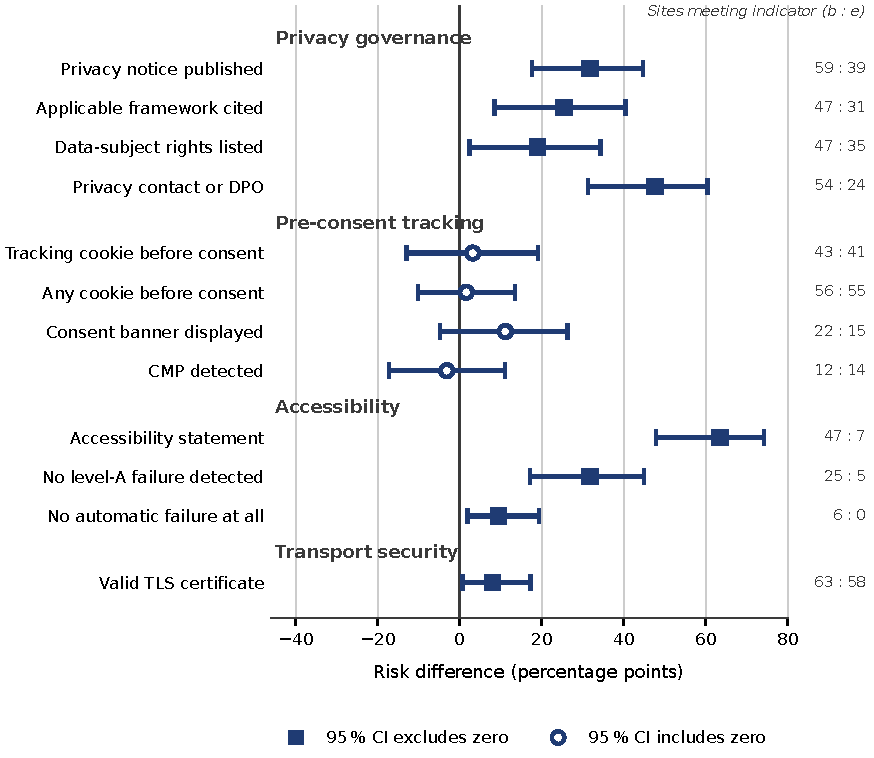
\includegraphics[width=\textwidth]{fig_forest.pdf}
	\caption{Diferencias de riesgo entre el grupo de referencia y el censo ecuatoriano, con intervalos de Newcombe al 95\,\%, agrupadas por dominio. Los cuadrados rellenos marcan los intervalos que excluyen el cero; los c\'irculos huecos, los que lo incluyen. A la derecha se indican los recuentos de sitios conformes sobre 63. Los valores positivos indican una proporci\'on mayor en el grupo de referencia.}\label{fig:forest}
\end{figure*}

\subsection{Gobernanza de la privacidad (PI1)}\label{sec:results-governance}

Las diferencias de gobernanza fueron las mayores y las m\'as robustas del estudio. Hab\'ia un aviso de privacidad alcanzable desde la portada en 59 de los 63 sitios del grupo de referencia (93,7\,\%) y en 39 de los 63 sitios ecuatorianos (61,9\,\%), una diferencia de 31,7 puntos porcentuales (raz\'on de momios 9,08; $p$ ajustada $<0{,}001$). La exigencia de que el aviso nombre un instrumento jur\'idico espec\'ifico redujo ambas cifras, al 74,6\,\% y al 49,2\,\% respectivamente (raz\'on de momios 3,03; $p$ ajustada $=0{,}045$).

La brecha m\'as amplia estuvo en la v\'ia por la que un interesado puede actuar. Se identific\'o un contacto de privacidad o delegado de protecci\'on de datos en el 85,7\,\% de los sitios del grupo de referencia y en el 38,1\,\% de los ecuatorianos, una diferencia de 47,6 puntos porcentuales (raz\'on de momios 9,75; $p$ ajustada $<0{,}001$). La enumeraci\'on de los derechos del interesado difiri\'o en la misma direcci\'on, 74,6\,\% frente a 55,6\,\%, pero esta diferencia no sobrevivi\'o a la correcci\'on por comparaciones m\'ultiples ($p$ ajustada $=0{,}235$) y aqu\'i se reporta solo como indicativa.

El desglose regional del grupo de referencia figura en la Tabla~\ref{tab:reg}. Debe leerse como descriptivo: con subgrupos de tres a cinco instituciones, el intervalo de Wilson en torno a una proporci\'on abarca m\'as de 50 puntos porcentuales, de modo que estos datos no pueden sostener ninguna ordenaci\'on regional. Con todo, merece la pena registrar dos patrones por ser grandes en relaci\'on con esa incertidumbre. Las instituciones chinas del grupo de referencia son las menos propensas a publicar un aviso de primer nivel, dos de seis, y ninguna public\'o declaraci\'on de accesibilidad; esa misma ausencia de declaraci\'on de accesibilidad se da en las cinco instituciones agrupadas como Resto de Asia, de modo que no es un rasgo exclusivo del subgrupo chino. Europa continental cita un marco jur\'idico en nueve de diez instituciones, pero las diez no son homog\'eneas en cuanto al instrumento aplicable: dos son suizas y est\'an sujetas a la Ley Federal de Protecci\'on de Datos revisada \citep{fadp_ch} y no al RGPD. De igual modo, las tres instituciones canadienses son entidades p\'ublicas regidas por leyes provinciales del sector p\'ublico \citep{fippa_on,fippa_bc,quebec_privacy}, y no por la Ley federal de Protecci\'on de la Informaci\'on Personal y los Documentos Electr\'onicos (PIPEDA) \citep{pipeda2000}, que se aplica a la actividad comercial, por lo que no cabe presumir un r\'egimen canadiense \'unico.

El c\'odigo parcial afecta a estas comparaciones de forma desigual, y su efecto se reporta aqu\'i para que no haya que inferirlo. Contar una celda parcial como cumplimiento del indicador en lugar de como incumplimiento deja inalterada la diferencia del contacto de privacidad en 47,6 puntos porcentuales, porque ese indicador no admite c\'odigo parcial, y mueve la diferencia de la declaraci\'on de accesibilidad menos de dos puntos, del 63,5 al 61,9. S\'i importa para los tres restantes. La diferencia del aviso cae de 31,7 a 27,0 puntos y la de los derechos sube de 19,0 a 27,0, en ambos casos sin alterar la conclusi\'on que de ellas se extrae. La diferencia del marco jur\'idico es la sensible: sube de 25,4 a 41,3 puntos, porque 11 de las 63 instituciones del grupo de referencia nombran un instrumento que no las gobierna, frente a 1 de las 63 instituciones ecuatorianas. Le\'ida de una u otra manera la brecha corre en la misma direcci\'on, pero la magnitud de la brecha del marco est\'a condicionada al tratamiento que se d\'e a un instrumento mal aplicado, y ninguna afirmaci\'on de este art\'iculo descansa en su tama\~no exacto.

Un indicador documental adicional queda registrado en el Ap\'endice~\ref{ap:mundo} y se reporta aqu\'i en lugar de compararse. Se hall\'o una pol\'itica de cookies espec\'ifica, que es un documento publicado y por tanto distinta de la medici\'on en vivo del banner de la Secci\'on~\ref{sec:results-cookies}, en 14 de las 63 instituciones del grupo de referencia (22,2\,\%). Se concentra en el Reino Unido, en 5 de 7 instituciones, y en Europa continental, en 4 de 10, y est\'a ausente en las seis instituciones chinas y en las cinco del grupo Resto de Asia. Se excluye de la Tabla~\ref{tab:comp} porque la matriz ecuatoriana no registra contrapartida, por lo que el indicador carece de grupo de comparaci\'on; se conserva en el ap\'endice porque es el complemento documental de la medici\'on en vivo y el lector puede querer relacionar ambas.

\begin{table*}[htbp]
	\centering
	\caption{Grupo de referencia por regi\'on: instituciones que cumplen cada indicador documental sobre el total regional. Los porcentajes y los intervalos se omiten deliberadamente: con $n$ entre 3 y 24 sugerir\'ian una precisi\'on que los datos no tienen.}\label{tab:reg}
	\small
	\begin{tabular}{@{}lccccc@{}}
		\toprule
		\textbf{Regi\'on} & \textbf{$n$} & \textbf{Aviso} & \textbf{Marco} & \textbf{Contacto/DPD} & \textbf{Accesibilidad} \\
		\midrule
		Estados Unidos & 24 & 24 & 17 & 23 & 22 \\
		Reino Unido & 7 & 7 & 4 & 5 & 7 \\
		Europa continental & 10 & 10 & 9 & 10 & 8 \\
		China & 6 & 2 & 2 & 3 & 0 \\
		RAE de Hong Kong & 3 & 3 & 3 & 2 & 3 \\
		Resto de Asia & 5 & 5 & 4 & 4 & 0 \\
		Australia & 5 & 5 & 5 & 4 & 4 \\
		Canad\'a & 3 & 3 & 3 & 3 & 3 \\
		\midrule
		\textbf{Total} & \textbf{63} & \textbf{59} & \textbf{47} & \textbf{54} & \textbf{47} \\
		\bottomrule
	\end{tabular}
\end{table*}

\subsection{Comportamiento previo al consentimiento (PI2)}\label{sec:results-cookies}

La Figura~\ref{fig:cookies} reporta las mediciones en vivo. Observados desde Ecuador, los dos grupos se comportaron de forma similar. Se fij\'o al menos una cookie antes de cualquier interacci\'on de consentimiento en el 88,9\,\% de los sitios del grupo de referencia y en el 87,3\,\% de los ecuatorianos; espec\'ificamente cookies de rastreo, en el 68,3\,\% y el 65,1\,\%. La diferencia en el indicador de rastreo fue de 3,2 puntos porcentuales a favor de Ecuador, con un intervalo al 95\,\% de $[-13{,}0, +19{,}1]$ puntos porcentuales y una $p$ ajustada de 1,000. Un aviso de consentimiento visible fue, en ambos grupos, un fen\'omeno minoritario (34,9\,\% y 23,8\,\%), y se detect\'o una plataforma de gesti\'on del consentimiento algo m\'as a menudo en Ecuador (22,2\,\%) que en el grupo de referencia (19,0\,\%), una diferencia bien dentro de la variaci\'on muestral.

Todas las cifras de esta secci\'on se calculan con la taxonom\'ia de cookies ampliada del Ap\'endice~\ref{ap:codebook}, como todo el art\'iculo. Con la lista original, el recuento de rastreo ecuatoriano ser\'ia de 40 de 63 en lugar de 41, una diferencia de un sitio, y el recuento del grupo de referencia quedar\'ia inalterado; ninguna conclusi\'on de esta secci\'on depende de esa elecci\'on.

\begin{figure*}[htbp]
	\centering
	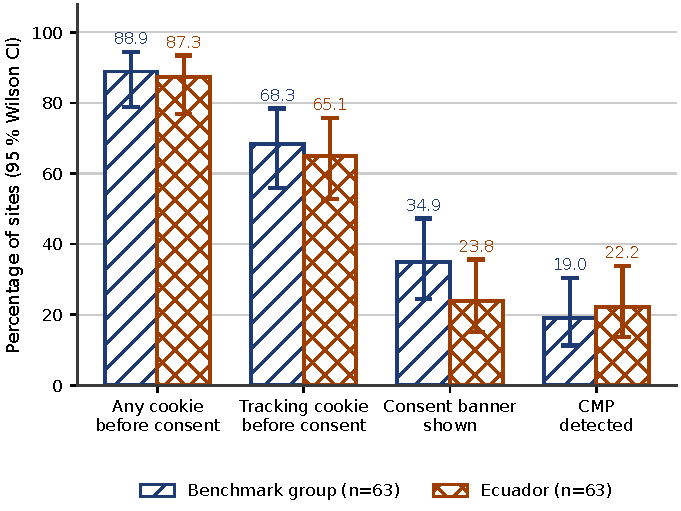
\includegraphics[width=\textwidth]{fig_cookies.pdf}
	\caption{Estado de las cookies registrado antes de cualquier interacci\'on con una interfaz de consentimiento, con intervalos de Wilson al 95\,\%. Todas las mediciones se tomaron desde un \'unico punto de observaci\'on en Ecuador en agosto de 2026; un visitante europeo no observar\'ia necesariamente el mismo comportamiento en los sitios europeos del grupo de referencia.}\label{fig:cookies}
\end{figure*}

La ausencia de una diferencia detectable no debe leerse como demostraci\'on de equivalencia. Con 63 sitios por grupo y una proporci\'on agrupada observada de 84/126 = 0,667, la menor diferencia que este dise\~no podr\'ia detectar con una potencia del 80\,\% y $\alpha=0{,}05$ bilateral es de 23,3 puntos porcentuales; detectar una diferencia verdadera del tama\~no aqu\'i observado exigir\'ia 3461 sitios por grupo. Dos pruebas unilaterales confirman el punto directamente: la equivalencia se rechaza con un margen de $\pm 10$ puntos porcentuales ($p=0{,}208$) y con $\pm 15$ ($p=0{,}079$), y solo se sostiene con un margen de $\pm 20$ ($p=0{,}023$), demasiado amplio para resultar sustantivamente interesante. Demostrar equivalencia dentro de $\pm 10$ puntos exigir\'ia, mediante dos pruebas unilaterales con $\alpha=0{,}05$ y potencia del 80\,\% y la misma proporci\'on agrupada, 275 sitios por grupo si la diferencia verdadera fuese exactamente nula y 590 si fuese del tama\~no aqu\'i observado, 3,2 puntos. El requisito depende de forma cr\'itica de un supuesto que estos datos no pueden fijar, raz\'on por la cual se ofrecen ambos valores. Las cuatro cantidades de este p\'arrafo las reproduce \verb|power_analysis.py| en el c\'odigo depositado. El enunciado correcto de este resultado es, por tanto, que \emph{el estudio no hall\'o evidencia de una diferencia en el rastreo previo al consentimiento, y careci\'o de potencia para establecer que los grupos son equivalentes}.

Una salvedad adicional y m\'as importante concierne a lo que un resultado nulo puede significar aqu\'i siquiera. Como todas las observaciones se tomaron desde Ecuador, la cifra del grupo de referencia confunde dos posibilidades que admiten lecturas jur\'idicas opuestas: que las instituciones europeas no condicionen sus interfaces de consentimiento a la ubicaci\'on del visitante y sencillamente rastreen a todo el mundo, o que s\'i las condicionen y muestren por tanto a un visitante europeo una interfaz distinta de la aqu\'i registrada. El presente dise\~no no puede distinguirlas, y la Secci\'on~\ref{sec:discussion} expone por qu\'e la distinci\'on importa y c\'omo deber\'ia resolverse.

\subsection{Accesibilidad declarada y seguridad del transporte (PI3, primera parte)}\label{sec:results-declared}

Publicaron una declaraci\'on de accesibilidad o un conjunto de herramientas de accesibilidad 47 de las 63 instituciones del grupo de referencia (74,6\,\%) y 7 de las 63 instituciones ecuatorianas (11,1\,\%), la mayor diferencia individual del estudio (raz\'on de momios 23,50; $p$ ajustada $<0{,}001$). Es plausible que deberes legales concretos expliquen parte de esa brecha: 22 de las 24 instituciones estadounidenses publican una declaraci\'on, en una jurisdicci\'on con la ADA y la Secci\'on 508 \citep{ada1990,section508}, y 8 de las 10 instituciones de Europa continental lo hacen al amparo de la Ley Europea de Accesibilidad \citep{eaa2019}. La cifra baja de Ecuador es coherente con el retraso regional documentado durante la \'ultima d\'ecada \citep{campoverdemolina2023accessibility,acostavargas2020dataset}.

La seguridad del transporte fue casi universal en ambos grupos: hab\'ia un certificado TLS v\'alido en los 63 sitios del grupo de referencia y en 58 de los 63 sitios ecuatorianos (92,1\,\%; $p$ ajustada $=0{,}288$). Subrayamos que este indicador mide \'unicamente la confidencialidad en tr\'ansito. Un sitio con una cadena de certificado impecable puede transmitir datos del visitante a cualquier n\'umero de terceros, y los cuatro indicadores previos al consentimiento de la Tabla~\ref{tab:comp} muestran precisamente ese patr\'on en ambos grupos.

La secci\'on de transparencia que la Ley Org\'anica de Transparencia y Acceso a la Informaci\'on P\'ublica (LOTAIP) exige a las entidades p\'ublicas ecuatorianas estaba presente en 47 de las 63 instituciones ecuatorianas (74,6\,\%). Se reporta aqu\'i por exhaustividad, dado que consta en el Ap\'endice~\ref{ap:ecuador}; no se emplea en ninguna comparaci\'on, puesto que carece de contrapartida en el grupo de referencia.

\subsection{Conformidad medida con las WCAG (PI3, segunda parte)}\label{sec:results-wcag}

La Tabla~\ref{tab:wcag} reporta los resultados de la auditor\'ia y la Figura~\ref{fig:wcag} la distribuci\'on de los nodos con fallo por nivel de conformidad.

\begin{table*}[htbp]
	\centering
	\caption{Resultados WCAG detectables autom\'aticamente (axe-core 4.13, agosto de 2026, solo la portada). Los porcentajes son de sitios salvo indicaci\'on contraria. El conjunto de reglas se especifica en la Secci\'on~\ref{sec:methods-audit}.}\label{tab:wcag}
	\small
	\begin{tabular}{@{}p{7.4cm}cc@{}}
		\toprule
		\textbf{Medida} & \textbf{Referencia} & \textbf{Ecuador} \\
		\midrule
		Mediana de reglas distintas incumplidas por sitio & 2 & 4 \\
		Sitios sin fallo autom\'atico en ning\'un nivel & 9,5\,\% & 0,0\,\% \\
		Sitios sin fallo autom\'atico de nivel A & 39,7\,\% & 7,9\,\% \\
		Enlaces sin nombre accesible (2.4.4, nivel A) & 23,8\,\% & 81,0\,\% \\
		Contraste insuficiente (1.4.3, nivel AA) & 25,4\,\% & 79,4\,\% \\
		Im\'agenes sin alternativa textual (regla \texttt{image-alt}, criterio de \'exito 1.1.1, nivel A) & 15,9\,\% & 30,2\,\% \\
		\midrule
		\multicolumn{3}{@{}l}{\textit{Distribuci\'on de los nodos con fallo por nivel, con todas las reglas habilitadas}}\\
		\quad Nivel A & 19\,\% & 45\,\% \\
		\quad Nivel AA & 22\,\% & 29\,\% \\
		\quad Nivel AAA & 60\,\% & 26\,\% \\
		\multicolumn{3}{@{}l}{\textit{La misma distribuci\'on excluyendo las reglas AAA y renormalizando}}\\
		\quad Nivel A & 46,0\,\% & 61,1\,\% \\
		\quad Nivel AA & 54,0\,\% & 38,9\,\% \\
		\bottomrule
	\end{tabular}
	\par\vspace{3pt}
	\footnotesize\RaggedRight\textit{Nota:} la mediana es de reglas distintas incumplidas, no de nodos con fallo. Los porcentajes por nivel son sobre el total de nodos con fallo de cada grupo y est\'an redondeados al entero m\'as pr\'oximo, raz\'on por la cual la distribuci\'on del grupo de referencia suma 101\,\%. El bloque renormalizado se calcula a partir de los recuentos de nodos sin redondear y no de los porcentajes redondeados que lo preceden, razón por la cual 19 y 22 dan 46,0 y 54,0 en lugar de 46,3 y 53,7.
\end{table*}

\begin{figure*}[htbp]
	\centering
	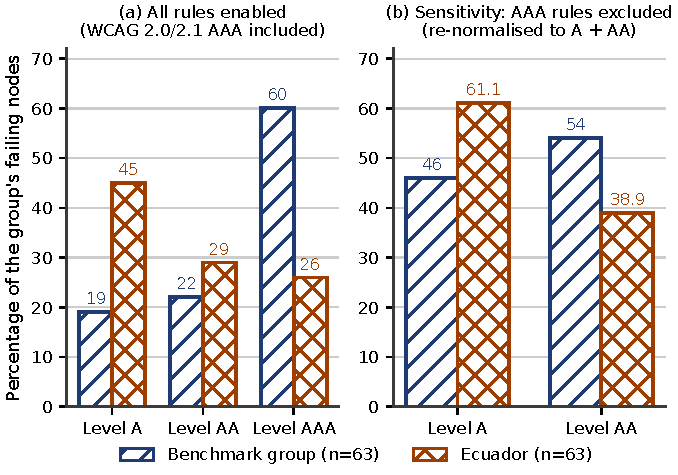
\includegraphics[width=\textwidth]{fig_wcag_levels.pdf}
	\caption{Distribuci\'on de los nodos con fallo por nivel de conformidad WCAG. El panel (a) usa el conjunto completo de reglas de este estudio, que incluye las reglas de nivel AAA de WCAG 2.0 y 2.1. El panel (b) las excluye y renormaliza sobre los niveles A y AA, y muestra que la ordenaci\'on de ambos grupos en el nivel A se conserva cuando no se cuenta la regla de contraste mejorado.}\label{fig:wcag}
\end{figure*}

Ninguno de los dos grupos obtuvo buenos resultados. Ning\'un sitio ecuatoriano y solo el 9,5\,\% de los sitios del grupo de referencia no produjeron fallo autom\'atico alguno en los niveles habilitados, y la mediana de reglas distintas incumplidas fue de cuatro en Ecuador frente a dos en el grupo de referencia. La distinci\'on que importa, sin embargo, es d\'onde recaen los fallos. En el grupo de referencia, el 19\,\% de los nodos con fallo estaba en el nivel A y el 60\,\% en el nivel AAA, este \'ultimo dominado por el contraste mejorado; en Ecuador, el 45\,\% estaba en el nivel A. Excluir por completo las reglas AAA y renormalizar sobre los niveles A y AA conserva la ordenaci\'on, 46,0\,\% frente a 61,1\,\% en el nivel A, lo que indica que el hallazgo cualitativo no es un artefacto de haber habilitado una \'unica regla exigente.

Dos lecturas que las cifras agregadas invitan a hacer no est\'an respaldadas por estos datos, y merece la pena descartar ambas expl\'icitamente porque un dise\~no que compara con un referente las propicia. \emph{No} es cierto que ninguna instituci\'on est\'e libre de fallos autom\'aticos: seis instituciones del grupo de referencia lo estaban. Y \emph{no} es cierto que el grupo de referencia falle solo en el nivel de la excelencia: el 60,3\,\% de sus sitios produjo al menos un fallo de nivel A, por lo que la mayor\'ia del grupo de referencia tampoco supera el escal\'on b\'asico. Lo que los datos respaldan es m\'as estrecho y sigue mereciendo reporte: los dos grupos difieren en la \emph{distribuci\'on} de sus fallos, no en la presencia de fallos.

El caso m\'as n\'itido es el criterio de \'exito 2.4.4, que exige que todo enlace tenga un texto que un lector de pantalla pueda anunciar; lo incumpli\'o el 81,0\,\% de los sitios ecuatorianos y el 23,8\,\% de los del grupo de referencia. El contraste insuficiente (1.4.3) sigui\'o el mismo patr\'on, 79,4\,\% frente a 25,4\,\%. El principio m\'as afectado en ambos grupos es la perceptibilidad, a trav\'es del contraste; Ecuador a\~nade un d\'eficit de operabilidad por enlaces y controles que en el grupo de referencia es marginal. Son los mismos tipos de error dominantes reportados para otros portales del sector p\'ublico \citep{iniesto2025service,aljedaani2025egovernment}.

Dos cautelas se aplican a las medidas basadas en niveles. Primera, la distribuci\'on de la Figura~\ref{fig:wcag}(a) se calcula sobre \emph{nodos} con fallo, que no son independientes dentro de un sitio: una \'unica plantilla con varios miles de elementos de bajo contraste puede dominar la distribuci\'on de su grupo. Segunda, la distribuci\'on es composicional, por lo que un grupo con m\'as fallos de nivel A ha de mostrar, aritm\'eticamente, una proporci\'on AAA menor. Ambas son razones para tratar la distribuci\'on por niveles como descriptiva; las medidas por sitio de la mitad superior de la Tabla~\ref{tab:wcag} son las inferencialmente seguras, y apuntan en la misma direcci\'on.

\subsection{Lo que encuentra la codificaci\'on manual exhaustiva y no encuentra la auditor\'ia automatizada (PI3, parte tres)}\label{sec:results-manual}

En los quince sitios de la submuestra, ninguno satisfizo los tres criterios de \'exito y once no satisficieron ninguno. El criterio 2.4.4 no se satisfizo en ninguno de los quince, el 1.1.1 en catorce de los quince y el 1.4.3 en doce. Toda fila que las reglas ACT remiten al juicio humano y que aun pod\'ia decidir un veredicto ha quedado resuelta, de modo que ninguna celda de la matriz de quince por tres queda abierta y los recuentos que siguen son completos y no cotas inferiores. La Tabla~\ref{tab:manual} da el detalle sitio a sitio junto al resultado automatizado de la misma p\'agina.

La comparaci\'on con la auditor\'ia automatizada es la sustancia de esta subsecci\'on. De las 45 celdas de sitio por criterio, la codificaci\'on exhaustiva bajo las reglas ACT encuentra fallos en 41. En 25 de esas 41 celdas, esto es en el 61\,\% de ellas, axe-core no hab\'ia reportado ninguna violaci\'on del criterio correspondiente en ese sitio. La carencia es mayor, y no menor, en el criterio cuya comprobaci\'on autom\'atica resulta m\'as familiar: en 1.1.1 la auditor\'ia automatizada no report\'o nada en 11 de los 14 sitios que fallan, y solo se\~nal\'o ese criterio en UTI, UTPL y NUS; en 2.4.4, en 8 de 15; y en 1.4.3, que un verificador automatizado calcula aritm\'eticamente, en 6 de 12.

Seis de los quince sitios no presentaban ning\'un fallo de nivel A bajo la auditor\'ia automatizada. Los seis incumplen a la vez el 1.1.1 y el 2.4.4, y ambos son criterios de nivel A, de modo que en todos los casos examinados la apariencia de cumplir el m\'inimo no sobrevivi\'o a una lectura elemento por elemento. Cuatro de los seis, Manchester, Northwestern, UC Berkeley y UCL, no produjeron ninguna violaci\'on automatizada en ning\'un nivel de conformidad, y esos cuatro est\'an entre las seis instituciones del grupo de referencia, el 9,5\,\% de ese grupo, que la Secci\'on~\ref{sec:results-wcag} reporta como libres de fallos automatizados. Manchester incumple los tres criterios examinados; los otros tres incumplen el 1.1.1 y el 2.4.4.

Nada de esto impugna al instrumento automatizado, que no est\'a dise\~nado para certificar conformidad. Cuantifica, sobre las p\'aginas que audita este estudio, lo que \citet{fischer2025coverage} establecen en general: los verificadores automatizados abordan una minor\'ia de los criterios de \'exito de las WCAG, de modo que superar una comprobaci\'on autom\'atica no es prueba de que un sitio sea accesible. La aportaci\'on de esta subsecci\'on es el tama\~no de esa brecha all\'i donde afecta al presente argumento. Para los tres criterios que le son m\'as centrales, seis de cada diez fallos de sitio por criterio son invisibles al instrumento automatizado, y la categor\'ia ``sin fallo de nivel A detectado'', que abarca 30 de los 126 sitios de este censo, no sobrevivi\'o al examen en ninguno de los seis casos en que se examin\'o.

\begin{table*}[htbp]
	\centering
	\caption{Resultado automatizado y codificaci\'on manual exhaustiva en los quince sitios de la submuestra de validaci\'on. Las tres columnas num\'ericas son recuentos de nodos con fallo reportados por axe-core 4.13.0 por nivel de conformidad el 14 de agosto de 2026. ``Se\~nalados'' indica cu\'ales de los tres criterios de \'exito lleg\'o a reportar la auditor\'ia automatizada. Las tres columnas de la derecha dan el veredicto de la codificaci\'on manual del 8 y 9 de septiembre de 2026, en la que un criterio no se satisface en un sitio si alg\'un elemento aplicable falla; ninguna celda queda abierta. La negrita marca las 25 celdas en las que la codificaci\'on manual encuentra fallos y la auditor\'ia automatizada no hab\'ia reportado ninguna violaci\'on de ese criterio. Los criterios 1.1.1 y 2.4.4 son de nivel A; el 1.4.3 es de nivel AA.}\label{tab:manual}
	\begin{tabular}{llrrrlccc}
		\toprule
		Sitio & Grupo & A & AA & AAA & Se\~nalados & 1.1.1 & 1.4.3 & 2.4.4 \\
		\midrule
		ECOTEC       & Ecuador &  0 &  6 & 27 & 1.4.3               & \textbf{no} & no          & \textbf{no} \\
		IAEN         & Ecuador &  2 &  1 &  2 & 1.4.3               & \textbf{no} & no          & \textbf{no} \\
		ULVR         & Ecuador & 11 &  2 &  0 & 1.4.3, 2.4.4        & \textbf{no} & no          & no          \\
		UNESUM       & Ecuador &  8 &  0 &  0 & 2.4.4               & \textbf{no} & \textbf{no} & no          \\
		UPS          & Ecuador & 10 &  0 &  0 & 2.4.4               & \textbf{no} & \textbf{no} & no          \\
		USECIPOL     & Ecuador &  0 &  0 &  4 & ninguno                & \textbf{no} & \textbf{no} & \textbf{no} \\
		UTI          & Ecuador &  9 & 10 &  1 & 1.1.1, 1.4.3, 2.4.4 & no          & no          & no          \\
		UTPL         & Ecuador &  9 &  1 & 25 & 1.1.1, 2.4.4        & no          & \textbf{no} & no          \\
		\midrule
		Cornell      & Referencia &  1 &  0 &  5 & ninguno                & s\'i         & \textbf{no} & \textbf{no} \\
		HKUST        & Referencia & 14 &  6 &  0 & 1.4.3, 2.4.4        & \textbf{no} & no          & no          \\
		Manchester   & Referencia &  0 &  0 &  0 & ninguno                & \textbf{no} & \textbf{no} & \textbf{no} \\
		NUS          & Referencia & 24 & 21 & 15 & 1.1.1, 1.4.3, 2.4.4 & no          & no          & no          \\
		Northwestern & Referencia &  0 &  0 &  0 & ninguno                & \textbf{no} & s\'i         & \textbf{no} \\
		UC Berkeley  & Referencia &  0 &  0 &  0 & ninguno                & \textbf{no} & s\'i         & \textbf{no} \\
		UCL          & Referencia &  0 &  0 &  0 & ninguno                & \textbf{no} & s\'i         & \textbf{no} \\
		\midrule
		\multicolumn{6}{l}{\emph{Sitios que no satisfacen el criterio}} & 14 / 15 & 12 / 15 & 15 / 15 \\
		\multicolumn{6}{l}{\emph{De esos, criterio no se\~nalado por la auditor\'ia automatizada}} & 11 & 6 & 8 \\
		\bottomrule
	\end{tabular}
\end{table*}

\subsection{\textquestiondown Concurren ambos compromisos? (PI4)}\label{sec:results-joint}

En el conjunto de los 126 sitios, la correlaci\'on de Spearman entre el n\'umero de nodos de accesibilidad con fallo y el n\'umero de cookies de rastreo previas al consentimiento es de 0,05. Ese coeficiente tiene un intervalo de confianza al 95\,\% de $[-0{,}13, +0{,}22]$ y $p=0{,}578$, y el dise\~no solo habr\'ia podido detectar una correlaci\'on de en torno a 0,25 con una potencia del 80\,\%. El coeficiente conjunto es por tanto compatible tanto con la ausencia de asociaci\'on como con una asociaci\'on positiva d\'ebil, y no puede sostener una afirmaci\'on de independencia.

El coeficiente conjunto es adem\'as el estimando equivocado, porque mezcla dos poblaciones cuyas distribuciones marginales difieren en ambas variables. La Tabla~\ref{tab:joint} ofrece la clasificaci\'on cruzada dentro de cada grupo de las dos medidas dicotomizadas. Dentro del grupo de referencia la asociaci\'on es, si acaso, ligeramente negativa (raz\'on de momios 0,54; $p$ de Fisher $=0{,}408$); dentro del grupo ecuatoriano est\'a esencialmente ausente (raz\'on de momios 1,27; $p$ de Fisher $=1{,}000$); la estimaci\'on de Mantel--Haenszel ajustada por grupo es 0,67. Ninguna de ellas es distinguible de la ausencia de asociaci\'on con este tama\~no muestral.

\begin{table*}[htbp]
	\centering
	\caption{Clasificaci\'on cruzada de la conformidad de nivel A detectable autom\'aticamente frente al rastreo previo al consentimiento, dentro de cada grupo. RM: raz\'on de momios de la conformidad dada la contenci\'on en el rastreo, con intervalo al 95\,\%.}\label{tab:joint}
	\small
	\begin{tabular}{@{}lcccccc@{}}
		\toprule
		\textbf{Grupo} & $A^{+}T^{-}$ & $A^{+}T^{+}$ & $A^{-}T^{-}$ & $A^{-}T^{+}$ & \textbf{RM [IC 95\,\%]} & \textbf{$p$} \\
		\midrule
		Referencia & 6 & 19 & 14 & 24 & 0,54 [0,17, 1,68] & 0,408 \\
		Ecuador & 2 & 3 & 20 & 38 & 1,27 [0,20, 8,21] & 1,000 \\
		\bottomrule
	\end{tabular}
	\par\vspace{3pt}
	\footnotesize\RaggedRight\textit{Nota:} $A^{+}$ sin fallo de nivel A detectable autom\'aticamente, $A^{-}$ al menos uno; $T^{-}$ sin cookie de rastreo antes del consentimiento, $T^{+}$ al menos una. La $p$ procede de la prueba exacta de Fisher bilateral. En Ecuador, 2 instituciones de 63 cumplieron ambos criterios. Bajo independencia cabr\'ia esperar $63 \times 0{,}079 \times 0{,}349 \approx 1{,}7$, de modo que esa cifra es exactamente lo que predice el azar y no aporta informaci\'on sobre acoplamiento.
\end{table*}

La conclusi\'on defendible de la PI4 es negativa, y merece enunciarse con precisi\'on porque la tentaci\'on es exagerarla. Estos datos no aportan evidencia de que las instituciones que invierten en accesibilidad contengan tambi\'en el rastreo, ni evidencia de lo contrario. No bastan para establecer que ambas cosas sean independientes; establecerlo exigir\'ia o bien una muestra sustancialmente mayor, o bien un par de medidas continuas con mayor potencia.

\subsection{\textquestiondown De qui\'en es la ubicaci\'on que determina la protecci\'on? (PI5)}\label{sec:results-vantage}

La replicaci\'on desde cuatro puntos de observaci\'on arroj\'o 121 de los 126 sitios medidos con \'exito en las tres pasadas de los cuatro puntos. Los cinco sitios que quedan fuera se nombran aqu\'i, porque un dise\~no pareado no puede imputarlos y el lector tiene derecho a saber cu\'ales son. Cada uno de ellos no lleg\'o a cargar en al menos una pasada, en todos los casos por agotamiento del tiempo de conexi\'on o por superarse el l\'imite de navegaci\'on de 45\,s, es decir, porque el servidor no respondi\'o y no porque la auditor\'ia se interrumpiera. Son la Universit\'e Paris-Saclay, que fall\'o en una pasada brit\'anica; la ESPOL, en dos pasadas alemanas; la UCSG, en dos pasadas ecuatorianas; la UDET, en una alemana y las tres brit\'anicas; y la UNEMI, en las tres ecuatorianas y una estadounidense. Cuatro de los cinco son ecuatorianos, lo que es en s\'i mismo un hallazgo sobre la disponibilidad de esos portales y se retoma en la Secci\'on~\ref{sec:threats}. Los 121 sitios retenidos comprenden 62 del grupo de referencia y 59 del censo ecuatoriano. Las tres magnitudes de control se comportaron como se requer\'ia: el n\'umero medio de violaciones WCAG por sitio fue de 3,53, 3,51, 3,54 y 3,50 en los puntos ecuatoriano, alem\'an, brit\'anico y estadounidense respectivamente, una dispersi\'on del 1,1\,\% entre los extremos, lo que confirma que las p\'aginas se renderizaron de forma id\'entica. El acuerdo entre pasadas en el indicador de rastreo, calculado por pares dentro de cada punto de observaci\'on sobre los 121 sitios, oscil\'o entre el 95,9\,\% y el 100\,\% a lo largo de los doce pares. Ese rango describe la estabilidad de la medida sobre las pasadas efectivamente ejecutadas; no establece que tres pasadas sean suficientes en general, y la regla de mayor\'ia se usa precisamente porque pasadas individuales discrepan en un n\'umero peque\~no de sitios.

El rastreo previo al consentimiento, en cambio, difiri\'o seg\'un la ubicaci\'on del visitante. Se observ\'o en 82 de los 121 sitios desde Ecuador (67,8\,\%; IC 95\,\% 59,0--75,4), en 79 desde Estados Unidos (65,3\,\%), en 76 desde el Reino Unido (62,8\,\%) y en 73 desde Alemania (60,3\,\%; 51,4--68,6). La $Q$ de Cochran sobre los cuatro puntos da $Q=15{,}88$, 3 grados de libertad, $p=0{,}0012$.

Las comparaciones pareadas de la Tabla~\ref{tab:vantage} localizan esa diferencia, y la pol\'itica de multiplicidad de la Secci\'on~\ref{sec:methods-stats} se aplica a las seis como familia. Ecuador difiere de Alemania, con 9 pares discordantes todos en la misma direcci\'on (exacta $p=0{,}0039$; $p$ ajustada por Holm $=0{,}023$), y ese contraste es el hallazgo de la secci\'on: es adem\'as el contraste que la Secci\'on~\ref{sec:methods-vantage} identific\'o como libre de todo artefacto de residencial frente a centro de datos. La diferencia entre Ecuador y el Reino Unido no sobrevive a la correcci\'on dentro de la familia (bruta $p=0{,}031$; ajustada $p=0{,}156$) y se reporta solo como indicativa. Ning\'un otro par es distinguible: el menor valor ajustado entre los cuatro restantes es 0,281, para Estados Unidos frente a Alemania.

La conclusi\'on no depende de esa regla de inclusi\'on. Exigir \'exito en las tres pasadas de todos los puntos de observaci\'on es el m\'as estricto de los tres criterios defendibles, y el an\'alisis se repiti\'o con los dos m\'as laxos. Exigir al menos dos pasadas v\'alidas por punto admite a Paris-Saclay y da $n=122$, con todos los recuentos de pares discordantes, todos los valores $p$ exactos y la $Q$ de Cochran id\'enticos a los de la Tabla~\ref{tab:vantage}. Exigir al menos una pasada v\'alida admite adem\'as a la UCSG y la ESPOL y da $n=124$, con lo que las marginales pasan a 84, 80, 78 y 74 sitios, la $Q$ de Cochran sube a 16,42 ($p=0{,}00093$) y el contraste Ecuador--Alemania se refuerza hasta diez pares discordantes, todos en la misma direcci\'on (exacta $p=0{,}0020$; $p$ ajustada por Holm $=0{,}012$). La UNEMI y la UDET no pueden admitirse bajo ninguna regla, dado que ninguna de las dos tiene una sola observaci\'on v\'alida en uno de los cuatro puntos. La ordenaci\'on de los cuatro puntos de observaci\'on y la significaci\'on del contraste Ecuador--Alemania son, por tanto, invariantes a esta elecci\'on, y se reporta la regla m\'as estricta por ser la m\'as conservadora.

En este art\'iculo aparecen tres cifras de rastreo para Ecuador que no son intercambiables, de modo que la relaci\'on entre ellas se enuncia aqu\'i en vez de dejarse al lector. La Tabla~\ref{tab:comp} reporta 41 de los 63 sitios ecuatorianos y 43 de los 63 del grupo de referencia, esto es 84 de los 126 en total (66,7\,\%), a partir de una \'unica pasada del 14 de agosto de 2026. La presente secci\'on reporta 82 de los 121 sitios observados con \'exito en todos los puntos (67,8\,\%), consolidados sobre tres pasadas del 15 de agosto de 2026. Ambas usan la taxonom\'ia ampliada, y las dos cifras difieren en conjunto de sitios, regla de consolidaci\'on y fecha, y ninguna sustituye a la otra: la primera sostiene la comparaci\'on entre grupos, la segunda la comparaci\'on dentro de cada sitio entre puntos de observaci\'on.

\begin{table*}[htbp]
	\centering
	\caption{Pruebas exactas de McNemar del rastreo previo al consentimiento entre puntos de observaci\'on ($n=121$ sitios observados en los cuatro). $a$: sitios con rastreo en ambos puntos; $b$: sitios con rastreo en el primero pero no en el segundo; $c$: el caso inverso; $d$: sitios sin rastreo en ninguno. Solo los pares discordantes aportan informaci\'on. $p_{\text{H}}$: ajustada por Holm sobre las seis comparaciones de esta familia.}\label{tab:vantage}
	\small
	\begin{tabular}{@{}lccccccc@{}}
		\toprule
		\textbf{Comparaci\'on} & $a$ & $b$ & $c$ & $d$ & \textbf{Discordantes} & \textbf{$p$} & \textbf{$p_{\text{H}}$} \\
		\midrule
		Ecuador frente a Alemania & 73 & 9 & 0 & 39 & 9 & 0,0039 & 0,023 \\
		Ecuador frente a Reino Unido & 76 & 6 & 0 & 39 & 6 & 0,031 & 0,156 \\
		Estados Unidos frente a Alemania & 72 & 7 & 1 & 41 & 8 & 0,070 & 0,281 \\
		Reino Unido frente a Alemania & 73 & 3 & 0 & 45 & 3 & 0,250 & 0,750 \\
		Ecuador frente a Estados Unidos & 79 & 3 & 0 & 39 & 3 & 0,250 & 0,750 \\
		Estados Unidos frente a Reino Unido & 75 & 4 & 1 & 41 & 5 & 0,375 & 0,750 \\
		\bottomrule
	\end{tabular}
	\par\vspace{3pt}
	\footnotesize\RaggedRight\textit{Nota:} las filas se ordenan por la $p$ bruta. Los totales marginales que la tabla implica son 82 sitios con rastreo desde Ecuador, 79 desde Estados Unidos, 76 desde el Reino Unido y 73 desde Alemania, que son los recuentos reportados en el texto.
\end{table*}

El mecanismo se hace visible en cuanto las cookies se atribuyen al proveedor que las fija. La Figura~\ref{fig:vantage} muestra la proporci\'on de sitios en que cada proveedor fij\'o al menos una cookie antes de cualquier interacci\'on de consentimiento. El 15 de agosto de 2026, tres proveedores no fijaron cookie alguna en los puntos de observaci\'on alem\'an y brit\'anico mientras que s\'i las fijaron en el ecuatoriano y el estadounidense, en las mismas p\'aginas y dentro de la misma pasada: Microsoft, cuyas cookies de Clarity, publicidad y Universal Event Tracking (UET) aparecieron en 14 sitios desde Ecuador y 14 desde Estados Unidos, y en ninguno desde Alemania o el Reino Unido; TapAd, en 4 y 4 sitios y en ninguno; y StackAdapt, en 2 y 2 sitios y en ninguno, un recuento demasiado peque\~no para sostener nada m\'as all\'a de su propia descripci\'on. El LinkedIn Insight Tag sigui\'o el mismo patr\'on de forma atenuada, en 14 y 14 sitios frente a 3 y 7. Google Analytics, Meta y Adobe redujeron su huella solo moderadamente y lo hicieron de forma similar en los cuatro puntos. Se trata de observaciones de conducta en una fecha; no son afirmaciones sobre lo que ning\'un proveedor decidi\'o o pretendi\'o.

\begin{figure*}[htbp]
	\centering
	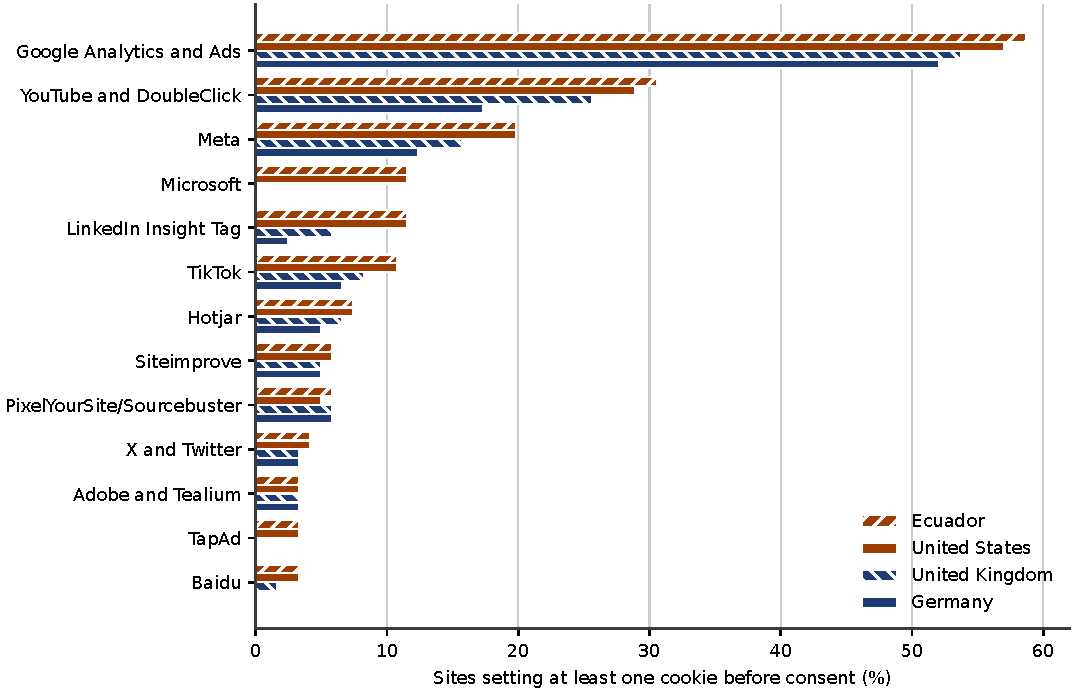
\includegraphics[width=\textwidth]{fig_vantage.pdf}
	\caption{Proporci\'on de sitios en que cada proveedor publicitario fij\'o al menos una cookie antes de cualquier interacci\'on de consentimiento, por punto de observaci\'on ($n=121$ sitios, mayor\'ia de tres pasadas, agosto de 2026). El color marca el per\'imetro que aplican los propios proveedores, no una frontera jur\'idica: azul marino para los dos puntos en que las cookies de proveedor quedaron suprimidas, Alemania y el Reino Unido, y ocre para los dos en que no, Ecuador y Estados Unidos. Que ese per\'imetro comercial incluya al Reino Unido, que est\'a fuera del Espacio Econ\'omico Europeo, es un hallazgo de la Secci\'on~\ref{sec:results-vantage} y no una premisa de la figura. Los proveedores se ordenan por su prevalencia vista desde Ecuador. Se muestran trece de las veintiuna familias de la taxonom\'ia del Ap\'endice~\ref{ap:codebook}. Se omiten seis por estar presentes en menos de cuatro sitios desde Ecuador, a saber, Privacy Sandbox, StackAdapt, Snapchat y ContentSquare en dos sitios cada una y Pinterest y Matomo en uno; las dos restantes, Quantcast y LiveIntent, no fijaron ninguna cookie coincidente en ning\'un sitio desde ning\'un punto de observaci\'on y est\'an por ello ausentes de la figura como resultado de la medici\'on y no de una elecci\'on de presentaci\'on.}\label{fig:vantage}
\end{figure*}

Dos rasgos de este patr\'on merecen \'enfasis porque no son los que predecir\'ia el encuadre institucional. Primero, la supresi\'on no se limita a las instituciones europeas: universidades ecuatorianas, chinas y estadounidenses que incrustan estas etiquetas dejan tambi\'en de fijar las cookies correspondientes cuando el visitante est\'a en Alemania o en el Reino Unido. El comportamiento pertenece por tanto al proveedor, no a la instituci\'on ni a la ley que la vincula. Segundo, la mayor\'ia de los proveedores trata al Reino Unido como interior al per\'imetro protegido pese a que ya no pertenece al Espacio Econ\'omico Europeo, lo que es coherente con que esos proveedores operen una lista de pa\'ises y no una prueba jur\'idica. TikTok y Baidu son las excepciones: ambos fijan sensiblemente m\'as cookies para los visitantes brit\'anicos que para los alemanes, 10 sitios frente a 8 y 2 frente a 0 respectivamente, de modo que el per\'imetro es espec\'ifico de cada proveedor y no com\'un.

Se aplica una salvedad. Las cookies no atribuibles a ning\'un proveedor publicitario tambi\'en descendieron en los puntos de observaci\'on europeo y brit\'anico, un 25,5\,\% y un 21,2\,\% respecto de Ecuador, mientras que el punto estadounidense difiri\'o solo un 0,8\,\%. Ese residuo es menor que la ca\'ida del 43,9\,\% y el 37,7\,\% de las cookies de proveedor y no afecta a los controles de renderizado, pero es probable que parte de \'el sea la cookie de gesti\'on de bots de Cloudflare y las cookies que fijan las propias plataformas de consentimiento, cuyo comportamiento tambi\'en var\'ia con la regi\'on del visitante. El residuo se reporta aqu\'i en lugar de ajustarse.

% =============================================================================
\section{Discusi\'on}\label{sec:discussion}
% =============================================================================

\subsection{Interpretaci\'on}\label{sec:discussion-interp}

Tres hallazgos sobreviven al an\'alisis de la Secci\'on~\ref{sec:results}, y son de distinta naturaleza.

El primero es una brecha de gobernanza que resulta grande, robusta a la correcci\'on por comparaciones m\'ultiples y consistente en cuatro indicadores. La carencia ecuatoriana no es principalmente la ausencia de documentos, sino la ausencia de los elementos que hacen accionable un documento: un instrumento nombrado, una enumeraci\'on de derechos y, sobre todo, una v\'ia identificada por la que una persona pueda ejercerlos. La brecha de 47,6 puntos en el contacto de privacidad es la cifra m\'as consecuente del estudio, porque un derecho sin canal no es ejercitable. Que las instituciones del grupo de referencia obtengan buenos resultados aqu\'i no es prueba de una \'etica superior; es la consecuencia esperable de reg\'imenes jur\'idicos que imponen el deber de forma expl\'icita, y sugiere que lo mismo es alcanzable en Ecuador a medida que la LOPDP y su reglamento entran en su fase de aplicaci\'on \citep{lopdp2021,reglamentolopdp2023}.

El segundo es una brecha de accesibilidad cuya propiedad interesante es su forma. Ambos grupos fallan; la mayor\'ia del grupo de referencia falla tambi\'en en el escal\'on b\'asico. Lo que difiere es que los fallos ecuatorianos se concentran en el nivel A, donde los remedios son baratos y bien conocidos, principalmente el texto accesible de los enlaces y un contraste adecuado, y donde las consecuencias para los usuarios de tecnolog\'ia de apoyo son m\'as graves. Es el hallazgo m\'as inmediatamente accionable del estudio y el \'unico sobre el que se puede actuar sin legislaci\'on nueva.

El tercero es un resultado nulo sobre el rastreo previo al consentimiento que debe reportarse como tal. Observado desde Ecuador, alrededor de dos tercios de las instituciones de ambos grupos fijan cookies de rastreo antes de cualquier interacci\'on de consentimiento. El estudio no hall\'o diferencia; tampoco tuvo potencia para establecer equivalencia, y la Secci\'on~\ref{sec:results-cookies} enuncia la cota de forma expl\'icita. El hallazgo que sobrevive no es, por tanto, \guillemotleft no hay brecha\guillemotright, sino \guillemotleft la brecha, si la hay, no es grande, y desde luego no va en la direcci\'on que predecir\'ia la ordenaci\'on reputacional de ambos grupos\guillemotright.

Una cuarta observaci\'on se sigue de la ausencia de asociaci\'on entre las dos barreras, y ata\~ne al marco con el que este art\'iculo comenz\'o. La Secci\'on~\ref{sec:related-a11y} motiv\'o medir conjuntamente la accesibilidad y el rastreo previo al consentimiento sobre la base de que ambos son costes que un servicio impone a quienes est\'an obligados a usarlo, y de que el dise\~no universal trata tales costes como propiedades del servicio y no del usuario. Si esa ra\'iz compartida fuese tambi\'en organizativa, las instituciones que invierten en una forma de acceso tender\'ian a contener la otra. Los datos no dan evidencia de que lo hagan. La unidad conceptual de las dos barreras no encuentra, por tanto, correspondencia en una unidad institucional, al menos no en el nivel de la portada ni en estas dos poblaciones. La lectura que preferimos no es que el marco falle, sino que es prescriptivo y no descriptivo: identifica lo que un servicio inclusivo tendr\'ia que hacer, y la ausencia de correlaci\'on mide la distancia entre esa exigencia y la pr\'actica actual, en la que la accesibilidad y el rastreo los gobiernan oficinas distintas, proveedores distintos y, como muestra la Secci\'on~\ref{sec:discussion-legal} para el segundo de ellos, a veces nadie dentro de la instituci\'on. Esta es una hip\'otesis que estos datos no pueden someter a prueba, y se ofrece como tal; lo que los datos s\'i establecen es que un compromiso institucional \'unico no puede inferirse de ninguna de las dos barreras por separado, lo cual es una consecuencia pr\'actica para quien pretenda auditar solo una de ellas.

\subsection{\'Ambito territorial y qui\'en lo aplica en realidad}\label{sec:discussion-legal}

Una explicaci\'on del comportamiento del grupo de referencia se sugiere de inmediato, y es err\'onea por partida doble: que la protecci\'on del RGPD se detiene en la frontera de la Uni\'on, de modo que un estudiante que consulta el portal de una universidad europea desde Ecuador queda tan expuesto como en un sitio nacional. Es err\'onea en derecho, y la replicaci\'on desde cuatro puntos de observaci\'on muestra que tambi\'en lo es de hecho, aunque no en la direcci\'on que ese encuadre predecir\'ia.

Primero, el punto jur\'idico. El art\'iculo 3(1) del RGPD se aplica al tratamiento en el contexto de las actividades de un establecimiento de un responsable en la Uni\'on \emph{con independencia de que el tratamiento tenga lugar en la Uni\'on o no}, y el Comit\'e Europeo de Protecci\'on de Datos (CEPD) ha confirmado que la ubicaci\'on del interesado es irrelevante para ese supuesto \citep{gdpr2016,edpb2019territorial}. Una universidad alemana o francesa que fija cookies de marketing en el navegador de un visitante situado en Ecuador act\'ua, por tanto, dentro del \'ambito material y territorial del Reglamento. El art\'iculo 3(2) extiende el Reglamento a los responsables no establecidos en la Uni\'on que ofrecen bienes o servicios a interesados \emph{que se encuentren en} la Uni\'on, de modo que ese supuesto s\'i depende de d\'onde est\'e el interesado y no de d\'onde est\'e el responsable. La objeci\'on m\'as acotada y defendible concierne a un instrumento distinto: el art\'iculo 5(3) de la Directiva sobre la privacidad y las comunicaciones electr\'onicas, seg\'un se haya transpuesto en cada pa\'is, se articula en torno al equipo terminal de un usuario, y la gu\'ia del CEPD sobre su \'ambito t\'ecnico es la referencia adecuada \citep{eprivacy2002,edpb2024eprivacy}.

La medici\'on muestra despu\'es algo que el encuadre institucional no anticipa. La protecci\'on s\'i var\'ia con la ubicaci\'on del visitante, y de forma sustancial, pero no son las universidades quienes var\'ian su comportamiento. Son los proveedores publicitarios incrustados en sus p\'aginas. Microsoft, en 14 sitios; TapAd, en 4; y StackAdapt, en 2, no fijaron cookie alguna en los puntos de observaci\'on alem\'an y brit\'anico y las fijaron con normalidad en el ecuatoriano y el estadounidense, y lo hicieron tanto en sitios de universidades ecuatorianas, chinas y estadounidenses como en los europeos. La instituci\'on es un espectador en esto: incrusta una etiqueta, y la l\'ogica de geolocalizaci\'on dentro de la etiqueta determina lo que el visitante recibe.

De ah\'i se siguen tres consecuencias que, juntas, constituyen la aportaci\'on m\'as original que este estudio puede hacer.

La primera es que el cumplimiento se est\'a ejecutando en la capa equivocada, y por un actor cuya posici\'on jur\'idica es m\'as fuerte de lo que sugiere el encuadre institucional. Un proveedor que fija sus propias cookies, para sus propios fines publicitarios y de medici\'on, y que decide con arreglo a su propia lista de pa\'ises si fijarlas o no, no act\'ua conforme a instrucciones documentadas de la universidad: est\'a determinando fines y medios. En \emph{Fashion ID}, el Tribunal de Justicia sostuvo que el operador de un sitio que incrusta un complemento de un tercero es corresponsable junto con el proveedor respecto de la recogida y la transmisi\'on de los datos de los visitantes. Que el operador no tenga acceso a esos datos es irrelevante para esa calificaci\'on \citep{cjeu2019fashionid}; el CEPD adopta la misma l\'inea para terceros incrustados que act\'uan para sus propios fines \citep{edpb2021controller}. La sentencia se dict\'o bajo la Directiva 95/46/CE, que era el derecho aplicable en su momento, y la atribuci\'on que establece tiene dos niveles: la corresponsabilidad cubre la recogida y la transmisi\'on, mientras que el proveedor es responsable \'unico de todo lo que haga con los datos a partir de ah\'i. Le\'ido as\'i, el problema de responsabilidad proactiva no es solo que la universidad no pueda demostrar el cumplimiento de una conducta que no observa. Es que un segundo responsable, con obligaciones propias en virtud de los art\'iculos 26 y 5(2), opera una lista de pa\'ises no publicada que ninguna autoridad de control est\'a examinando.

La segunda es que la frontera es comercial, no jur\'idica. El Reino Unido abandon\'o el Espacio Econ\'omico Europeo, pero la mayor\'ia de los proveedores lo sigue situando dentro del per\'imetro protegido, mientras que TikTok y Baidu no. La protecci\'on de una persona depende por tanto de qu\'e listas de pa\'ises mantengan unas empresas privadas, y esas listas no se publican, ni est\'an armonizadas, ni se someten al escrutinio que recibir\'ia un instrumento jur\'idico.

La tercera es distributiva, y es el punto que conecta este hallazgo con la preocupaci\'on por el acceso universal con que se abri\'o este art\'iculo. La poblaci\'on que no recibe protecci\'on alguna es la situada fuera del per\'imetro de los proveedores, que incluye a todo el conjunto de aspirantes internacionales de Am\'erica Latina, \'Africa y buena parte de Asia. A un aspirante ecuatoriano que navega por las p\'aginas de admisi\'on de una universidad alemana se le rastrea; a un aspirante alem\'an que navega por las p\'aginas de una universidad ecuatoriana, no. La asimetr\'ia corre en la direcci\'on que agrava la desigualdad existente, y resulta invisible para cualquier ejercicio de vigilancia realizado desde dentro del per\'imetro, que es donde se sit\'uan los reguladores, los auditores y la mayor\'ia de los investigadores. Esta es precisamente la exclusi\'on por posici\'on geopol\'itica y econ\'omica que \citet{abascal2016rethinking} sostienen que la accesibilidad universal debe abordar junto a la exclusi\'on por capacidad, y aqu\'i aparece en una forma inusualmente tratable: el per\'imetro es una lista de pa\'ises, por lo que la poblaci\'on excluida puede enumerarse y la frontera puede medirse.

\subsection{Implicaciones para la pr\'actica}\label{sec:discussion-practice}

Para las instituciones ecuatorianas, la ordenaci\'on que estos resultados implican es inusualmente clara. La primera actuaci\'on es identificar un contacto de privacidad por cargo y direcci\'on en el aviso de primer nivel; es la intervenci\'on m\'as barata de la lista y cierra la mayor brecha. La segunda es nombrar el instrumento aplicable y enumerar los derechos que confiere la LOPDP, junto con el procedimiento para ejercerlos, sustituyendo las referencias gen\'ericas a \guillemotleft la legislaci\'on aplicable\guillemotright. La tercera es subsanar los fallos de accesibilidad de nivel A, empezando por el texto de los enlaces y el contraste, que juntos representan la mayor\'ia de los nodos de nivel A observados. La cuarta, y la menos urgente a la vista de la evidencia recogida, es la interfaz de consentimiento: a\~nadir un banner sin configurarlo para bloquear antes del consentimiento cambia el indicador medido sin cambiar la exposici\'on del usuario, una sustituci\'on que la literatura de medici\'on ha documentado repetidamente \citep{sanchezrola2019can,bollinger2022automating} y que los presentes datos no permiten descartar en ninguno de los dos grupos.

Para las instituciones del grupo de referencia, lo pertinente es que el 60,3\,\% de ellas produce al menos un fallo de nivel A, y que dos tercios fijan cookies de rastreo antes del consentimiento cuando se las observa desde fuera de la Uni\'on. La posici\'on reputacional no es prueba de desempe\~no ni en accesibilidad ni en privacidad. Una implicaci\'on adicional se sigue de la Secci\'on~\ref{sec:results-vantage} y se aplica a todas las instituciones de ambos grupos: un administrador que prueba su propio sitio desde su propia oficina solo ve lo que su ubicaci\'on le permite ver. Verificar lo que experimenta un aspirante internacional exige probar desde la regi\'on de ese aspirante, lo que no es dif\'icil ni costoso y, a la vista de esta evidencia, no se est\'a haciendo.

\subsection{Implicaciones para la pol\'itica p\'ublica}\label{sec:discussion-policy}

De aqu\'i se siguen dos implicaciones para los reguladores. Primera, para la autoridad ecuatoriana de protecci\'on de datos, los indicadores que separan con m\'as nitidez a los dos grupos son exactamente los verificables a bajo coste desde fuera de la instituci\'on, de modo que una autoevaluaci\'on supervisada peri\'odica contra una matriz publicada es administrativamente factible; el libro de c\'odigos del Ap\'endice~\ref{ap:codebook} se ofrece con ese prop\'osito. El riesgo que ello conlleva es bien conocido y conviene anticiparlo: un indicador que se convierte en objetivo se satisface en la superficie, y el banner de cookies es el caso m\'as claro de indicador que puede cumplirse sin cambio alguno de comportamiento.

Segunda, el patr\'on documentado en la Secci\'on~\ref{sec:results-vantage} concierne a las autoridades de control europeas y no a las ecuatorianas, y plantea una pregunta que la supervisi\'on tal como se practica hoy no formula. Cuando el cumplimiento del art\'iculo 5(3) por parte de un responsable lo entrega de facto la l\'ogica de geolocalizaci\'on de un tercero, el responsable no puede demostrar la responsabilidad proactiva del art\'iculo 5(2) respecto de una conducta que ni configur\'o ni observa. Una comprobaci\'on de supervisi\'on realizada desde dentro del per\'imetro hallar\'a conforme a ese responsable. Sugerimos que las auditor\'ias del comportamiento de consentimiento se realicen de forma rutinaria desde fuera del Espacio Econ\'omico Europeo, y que las listas de pa\'ises que operan los principales proveedores de etiquetas se traten como objeto supervisable por derecho propio.

\subsection{Amenazas a la validez}\label{sec:threats}

\emph{Validez de constructo.} El rastreo previo al consentimiento se mide de manera uniforme en once jurisdicciones cuyas obligaciones difieren radicalmente; en Estados Unidos no existe un deber general de consentimiento previo, y el derecho ecuatoriano no incorpora un equivalente del art\'iculo 5(3) de la Directiva sobre la privacidad y las comunicaciones electr\'onicas. El Ap\'endice~\ref{ap:mapeo} pone cada indicador en correspondencia con la obligaci\'on concreta, si la hay, en cada jurisdicci\'on, y los resultados de la Secci\'on~\ref{sec:results-cookies} se enuncian como conducta observada y no como hallazgos de cumplimiento. \guillemotleft Sin fallo de nivel A detectado\guillemotright{} es una afirmaci\'on sobre el subconjunto comprobable por m\'aquina y no una declaraci\'on de conformidad \citep{fischer2025coverage}. La seguridad del transporte se reporta separadamente de la protecci\'on de datos por la raz\'on dada en la Secci\'on~\ref{sec:results-declared}. La medici\'on basada en cookies deja fuera adem\'as \verb|localStorage|, \verb|IndexedDB|, las t\'ecnicas de huella digital, los p\'ixeles sin cookie y el etiquetado del lado del servidor, por lo que las cifras de rastreo aqu\'i reportadas son cotas inferiores.

\emph{Validez interna.} El grupo de referencia es un estrato de \'elite, no una muestra del mundo, por lo que los efectos de recursos y de jurisdicci\'on quedan completamente confundidos; no se midi\'o un tercer estrato. No se registraron variables de confusi\'on que habr\'ian podido registrarse, en particular el presupuesto, la matr\'icula, el idioma del sitio, el sistema de gesti\'on de contenidos y el proveedor de alojamiento, y este \'ultimo es una fuente plausible de falta de independencia dentro del grupo ecuatoriano, donde las plantillas compartidas son frecuentes. El tipo de instituci\'on registrado en el Ap\'endice~\ref{ap:ecuador}, p\'ublica, cofinanciada o autofinanciada, no se analiza aqu\'i.

\emph{Fiabilidad.} La codificaci\'on documental se realiz\'o sin doble codificaci\'on y sin coeficiente de fiabilidad entre codificadores. El subestudio de verificaci\'on de la Secci\'on~\ref{sec:methods-coding} hall\'o dos errores en 24 celdas reexaminadas; como esas celdas se seleccionaron de forma intencional, la cifra no es cota superior ni inferior de la tasa de error de la matriz completa, y se reporta solo como evidencia de que la tasa no es despreciable. La codificaci\'on de elementos que exigen juicio en varios idiomas, entre ellos el chino, el japon\'es, el coreano, el alem\'an, el franc\'es y el sueco, es la parte m\'as expuesta del dise\~no. La asimetr\'ia con las mediciones en vivo es en s\'i misma una limitaci\'on: la geolocalizaci\'on se verific\'o 84 veces y el estado de las cookies se consolid\'o sobre tres pasadas, mientras que cada celda documental descansa en una lectura \'unica de un solo codificador. Los c\'odigos parciales se trataron como incumplimiento, convenci\'on que penaliza a las instituciones con avisos segmentados; los porcentajes no se recalcularon con la convenci\'on alternativa. Los c\'odigos de sitios no verificables permanecieron en el denominador, lo que deprime espec\'ificamente los porcentajes ecuatorianos, dado que todos esos casos se dan en ese grupo.

\emph{Artefactos del punto de observaci\'on.} Los tres puntos no ecuatorianos se alcanzaron a trav\'es de una VPN comercial y sus direcciones de salida pertenecen a centros de datos, por lo que proveedores que traten de otro modo tales direcciones podr\'ian, en principio, imitar un efecto de ubicaci\'on. Tres observaciones acotan esa preocupaci\'on: los controles de renderizado fueron id\'enticos entre puntos con un margen del 1,1\,\%; los extremos alem\'an y estadounidense comparten tipo de red, de modo que su contraste est\'a libre del artefacto; y un extremo alem\'an se sustituy\'o por un segundo proveedor en un sistema aut\'onomo distinto con resultado indistinguible. Una preocupaci\'on sim\'etrica se aplica al punto ecuatoriano, que es el \'unico residencial: la exposici\'on all\'i observada podr\'ia ser una propiedad del operador de acceso concreto y no del pa\'is. Esto se someti\'o a prueba de forma directa. El protocolo completo se repiti\'o sobre los 126 sitios desde un segundo operador residencial ecuatoriano, en un sistema aut\'onomo distinto y en otra ciudad, con tres pasadas consolidadas por la misma regla de mayor\'ia. De los 124 sitios retenidos bajo ambos operadores, 82 (66,1\,\%) fijaron al menos una cookie de rastreo antes del consentimiento bajo el segundo operador, frente a 84 (67,7\,\%) bajo el primero. Hay 122 sitios concordantes y 2 discordantes, ambos en la misma direcci\'on, con una $p$ exacta de McNemar de 0,50. El acuerdo se mantiene por separado dentro de cada grupo, con una diferencia de 1,6 puntos porcentuales en ambos. Esta comparaci\'on no separa el operador de la fecha de observaci\'on, porque la segunda serie se recogi\'o tres semanas despu\'es, y los dos sitios discordantes son m\'as compatibles con un cambio en esos sitios que con un efecto de red. Dentro de ese l\'imite, el resultado ecuatoriano no es una propiedad de una sola red de acceso. La ca\'ida residual de cookies ajenas a los proveedores en los puntos europeo y brit\'anico, reportada en la Secci\'on~\ref{sec:results-vantage}, no queda plenamente explicada y es el punto m\'as d\'ebil de esta parte del dise\~no. Los cuatro puntos de observaci\'on se midieron adem\'as en un \'unico d\'ia, por lo que la replicaci\'on describe el comportamiento de los proveedores en esa fecha. Una limitaci\'on adicional concierne a qu\'e sitios pudo retener la replicaci\'on. Cinco de los 126 no respondieron en al menos una de las doce pasadas y quedan excluidos del an\'alisis pareado, y cuatro de esos cinco son ecuatorianos; la p\'erdida no es por tanto aleatoria respecto del grupo, y apunta en la direcci\'on de una menor disponibilidad de los portales ecuatorianos. Como el an\'alisis de sensibilidad reportado en la Secci\'on~\ref{sec:results-vantage} deja inalterada la conclusi\'on, el efecto sobre la comparaci\'on entre puntos es despreciable, pero la propia disponibilidad diferencial merece registrarse como observaci\'on sobre la infraestructura de ambos grupos.

\emph{Estabilidad de la medici\'on.} La revisi\'on documental sigue siendo una observaci\'on \'unica. El estado de las cookies previas al consentimiento no es determinista: depende de pruebas A/B, de subastas publicitarias, del nodo de la red de distribuci\'on de contenidos (CDN) y del momento del despliegue. Para la auditor\'ia en vivo esto se abord\'o con las tres pasadas por punto de observaci\'on, cuyo acuerdo entre pasadas oscil\'o entre el 95,9\,\% y el 100\,\%; para la comparaci\'on entre grupos de la Secci\'on~\ref{sec:results-cookies}, que descansa en la medici\'on de pasada \'unica de agosto, no. Solo se audit\'o la portada, mientras que la conformidad con las WCAG se define sobre p\'aginas y procesos completos, y las rutas transaccionales que este art\'iculo invoca como motivaci\'on, la admisi\'on y la matr\'icula, no se midieron en absoluto. Los detectores de banner y de CMP son heur\'isticos cuyas tasas de falsos negativos se desconocen.

\emph{Validez de la conclusi\'on estad\'istica.} Doce comparaciones se corrigieron por el procedimiento de Holm y solo los valores ajustados se emplean para sostener afirmaciones; el desglose regional se reporta sin inferencia por la raz\'on dada en la Secci\'on~\ref{sec:results-governance}. Los m\'argenes de equivalencia del an\'alisis TOST no se preespecificaron. La distribuci\'on de accesibilidad en el plano de los nodos est\'a sujeta a pseudorreplicaci\'on y a restricci\'on composicional, seg\'un se indica en la Secci\'on~\ref{sec:results-wcag}. Los recuentos de fallos no se normalizaron por la complejidad de la p\'agina, por lo que un portal grande acumular\'a m\'as nodos con fallo que uno peque\~no sin ser necesariamente menos accesible.

\emph{Validez externa.} Todas las observaciones se tomaron en una fecha y desde un pa\'is, y los resultados describen el estado de 126 portadas en agosto de 2026. El contenido web cambia; ninguna afirmaci\'on de este art\'iculo debe leerse como propiedad duradera de instituci\'on alguna.

% =============================================================================
\section{Conclusiones y trabajo futuro}\label{sec:conclusions}
% =============================================================================

Medidas frente a un grupo de referencia de 63 universidades de primer nivel, las 63 IES ecuatorianas mostraron sus brechas m\'as amplias y robustas en la gobernanza de la privacidad, sobre todo en la identificaci\'on de un contacto de privacidad (38,1\,\% frente a 85,7\,\%) y en la publicaci\'on de un aviso de privacidad de primer nivel (61,9\,\% frente a 93,7\,\%). En accesibilidad fallaron ambos grupos, pero los fallos se distribuyeron de forma distinta: el 45\,\% de los nodos con fallo ecuatorianos estaba en el nivel b\'asico A frente al 19\,\% del grupo de referencia, una ordenaci\'on que se conserva al excluir las reglas de nivel AAA. En el rastreo previo al consentimiento, observado desde Ecuador, el estudio no hall\'o diferencia entre los grupos y careci\'o de potencia para establecer que sean equivalentes. Dentro de cada grupo, la accesibilidad medida y la contenci\'on observada en el rastreo no resultaron asociadas.

Replicar la auditor\'ia en vivo desde cuatro puntos de observaci\'on estableci\'o despu\'es que la exposici\'on previa al consentimiento var\'ia con la ubicaci\'on del visitante y no con la de la instituci\'on. El 15 de agosto de 2026, las mismas 121 p\'aginas fijaron cookies de rastreo en el 67,8\,\% de las visitas desde Ecuador y en el 60,3\,\% de las visitas desde Alemania ($Q$ de Cochran, $p=0{,}0012$; Ecuador--Alemania, $p$ ajustada por Holm $=0{,}023$ sobre las seis comparaciones por pares), y la supresi\'on la ejecutaron los proveedores publicitarios: Microsoft, en 14 sitios; TapAd, en 4; y StackAdapt, en 2, no fijaron nada en los puntos alem\'an y brit\'anico mientras fijaban cookies en el ecuatoriano y el estadounidense sobre las mismas p\'aginas, incluidos sitios de universidades ecuatorianas y chinas.

Estos hallazgos sostienen una conclusi\'on pr\'actica, otra jur\'idica y otra distributiva. La conclusi\'on pr\'actica es que las carencias distintivas de Ecuador est\'an en la gobernanza y en la accesibilidad de nivel b\'asico, y ambas son subsanables sin legislaci\'on nueva. La conclusi\'on jur\'idica es que un deber que el derecho europeo impone a la universidad lo est\'an cumpliendo en la pr\'actica proveedores publicitarios que son ellos mismos responsables del tratamiento, con arreglo a listas de pa\'ises no publicadas, lo que satisface al visitante de Fr\'ancfort mientras deja a ninguna de las dos partes en posici\'on de rendir cuentas de forma demostrable: la universidad no puede responder de una conducta que no observa, y las obligaciones propias del proveedor no est\'an siendo supervisadas. La conclusi\'on distributiva es la que devuelve este art\'iculo a su punto de partida: los aspirantes que no reciben protecci\'on alguna son los situados fuera del per\'imetro que describen esas listas, es decir, la mayor parte del conjunto mundial de aspirantes internacionales, y su exposici\'on es invisible para quien pruebe desde dentro de \'el.

De las amenazas enunciadas en la Secci\'on~\ref{sec:threats} se siguen cuatro tareas adicionales: doble codificaci\'on independiente de al menos el 30\,\% de la muestra con una $\kappa$ de Cohen por indicador y reconciliaci\'on completa de las discrepancias; ampliaci\'on de la auditor\'ia a al menos cinco p\'aginas por sitio, incluida una ruta de admisi\'on o matr\'icula, con la p\'agina como unidad y el sitio como efecto aleatorio; medidas de rastreo m\'as robustas que la cookie, en particular el recuento de dominios de terceros distintos contactados antes del consentimiento; y un an\'alisis interno del grupo ecuatoriano por tipo de instituci\'on, tama\~no y plataforma, para el cual la variable necesaria ya consta en el Ap\'endice~\ref{ap:ecuador} y que probablemente tenga mayor valor local que cualquier comparaci\'on internacional. A ellas los presentes resultados a\~naden una quinta: cartografiar las listas de pa\'ises que operan los principales proveedores de etiquetas, midiendo desde un punto de observaci\'on por cada jurisdicci\'on candidata, para que el per\'imetro dentro del cual se entrega la protecci\'on pueda describirse emp\'iricamente en lugar de suponerse coincidente con frontera jur\'idica alguna.

\backmatter

\bmhead{Informaci\'on complementaria}

El script de auditor\'ia, su configuraci\'on, la salida en bruto por sitio en Notaci\'on de Objetos de JavaScript (JSON) de las doce pasadas multipunto junto con los registros de verificaci\'on de ubicaci\'on, el inventario completo de cookies con su clasificaci\'on bajo ambas taxonom\'ias, la matriz documental, el libro de c\'odigos y los cuadernos de an\'alisis est\'an depositados en un repositorio p\'ublico \citep{deposito2026}. Toda figura reportada en la Secci\'on~\ref{sec:results-vantage}, incluida la atribuci\'on por proveedor, es reproducible a partir de esos ficheros con el script de an\'alisis publicado junto a ellos.

\bmhead{Agradecimientos}

Los autores agradecen a los revisores cuyos comentarios sobre versiones sucesivas de este art\'iculo motivaron la replicaci\'on multipunto reportada en la Secci\'on~\ref{sec:results-vantage}.

\section*{Declaraciones}

\bmhead{Financiaci\'on}

No se recibi\'o financiaci\'on para la realizaci\'on de este estudio.

\bmhead{Intereses en competencia}

El autor de correspondencia y el tercer autor est\'an afiliados a la Universidad T\'ecnica Estatal de Quevedo, que es una de las 63 instituciones ecuatorianas evaluadas en este estudio y figura en el Ap\'endice~\ref{ap:ecuador}. La segunda autora est\'a afiliada al Ministerio de Educaci\'on del Ecuador, entidad p\'ublica del mismo sistema nacional de educaci\'on. Los autores participaron en este estudio como investigadores individuales y no en nombre de ninguna de las dos instituciones. Ninguna instituci\'on propuso, encarg\'o, financi\'o ni aprob\'o el trabajo, y ninguna tuvo papel alguno en su dise\~no, en la recogida o codificaci\'on de datos, en el an\'alisis ni en la decisi\'on de publicar. La codificaci\'on de la propia instituci\'on de los autores sigue el mismo libro de c\'odigos que cualquier otro sitio y se reporta en el Ap\'endice~\ref{ap:ecuador} sin excepci\'on.

\bmhead{Contribuciones de los autores}

G.G.-U.: conceptualizaci\'on, metodolog\'ia, software, an\'alisis formal, investigaci\'on, visualizaci\'on, recursos, curaci\'on de datos, administraci\'on del proyecto, supervisi\'on, redacci\'on --- borrador original, redacci\'on --- revisi\'on y edici\'on. A.Z.P.: investigaci\'on, curaci\'on de datos, validaci\'on, redacci\'on --- revisi\'on y edici\'on. E.D.-M.: investigaci\'on, software, validaci\'on, redacci\'on --- revisi\'on y edici\'on. Todos los autores leyeron y aprobaron el manuscrito final. No se declara papel de captaci\'on de financiaci\'on, dado que el estudio no recibi\'o financiaci\'on.

\bmhead{Disponibilidad de los datos}

Los conjuntos de datos generados y analizados durante el presente estudio est\'an disponibles de forma abierta en el repositorio Zenodo \citep{deposito2026}, bajo el Identificador de Objeto Digital de concepto \path{10.5281/zenodo.22405998}, que resuelve a la versi\'on m\'as reciente. El dep\'osito est\'a licenciado CC BY 4.0 para los datos y la documentaci\'on, y MIT para el c\'odigo.

\bmhead{Disponibilidad del c\'odigo}

El script de auditor\'ia y el c\'odigo de an\'alisis est\'an disponibles en el mismo repositorio \citep{deposito2026}, bajo licencia MIT.

\bmhead{Aprobaci\'on \'etica y consentimiento para participar}

No procede. El estudio analiz\'o p\'aginas web de acceso p\'ublico y no implic\'o participantes humanos, ni animales, ni datos personales.

\bmhead{Uso de inteligencia artificial generativa}

Durante la preparaci\'on y revisi\'on de este art\'iculo se utiliz\'o un asistente de inteligencia artificial generativa, y su papel se enuncia aqu\'i en t\'erminos espec\'ificos. Se emple\'o para redactar y revisar prosa en las secciones de m\'etodos, resultados y discusi\'on, en las leyendas de los ap\'endices y en la documentaci\'on y el texto de justificaci\'on por fila del dep\'osito; para escribir y corregir scripts auxiliares, a saber, la extracci\'on de la matriz documental a partir del fuente del art\'iculo, los c\'alculos de potencia y tama\~no muestral de la Secci\'on~\ref{sec:results-cookies} y una utilidad de normalizaci\'on, todos ellos publicados en el dep\'osito; para recalcular cantidades reportadas a partir de los datos depositados como comprobaci\'on del manuscrito; y para verificar fuentes bibliogr\'aficas y jur\'idicas contra sus originales. Se registra expl\'icitamente una excepci\'on: de los 349 elementos de imagen que la regla \texttt{qt1vmo} remite al juicio humano, 345 se resolvieron con su asistencia y fueron revisados por el primer autor, y los cuatro restantes los resolvi\'o el primer autor por s\'i solo; ambos grupos se identifican en el dep\'osito por su c\'odigo de evaluador, y el grupo asistido queda excluido de las estimaciones de acuerdo entre codificadores, que descansan \'unicamente en las codificaciones humanas independientes. Con esa excepci\'on, no se emple\'o para recoger datos, para operar el instrumento de auditor\'ia, para seleccionar o interpretar observaciones, ni para decidir lo que el estudio concluye. El instrumento de auditor\'ia es software convencional: axe-core 4.13.0 gobernado por Playwright 1.62.1 sobre Node.js v24.18.1 en las pasadas automatizadas, y los recolectores de consola \texttt{act\_recode.js} y \texttt{act\_images.js} en las rondas por elemento, con el an\'alisis en Python 3.10.3 mediante NumPy 2.2.6, SciPy 1.15.3 y Matplotlib 3.10.9. Ninguna medici\'on, tabla o figura fue generada por el asistente. Cada cantidad que recalcul\'o se reconcili\'o contra los ficheros depositados, y all\'i donde una cifra reportada no pudo reproducirse se corrigi\'o el manuscrito en lugar de aceptar el c\'alculo. Los autores revisaron toda esa salida, la verificaron contra las fuentes primarias y los datos depositados, y asumen la plena responsabilidad del contenido de este art\'iculo.

% =============================================================================
\clearpage
\onecolumn
\begin{appendices}
% =============================================================================

\renewcommand{\thetable}{\thesection\arabic{table}}
\renewcommand{\thefigure}{\thesection\arabic{figure}}

\section{Libro de c\'odigos y definiciones operativas}\label{ap:codebook}
\setcounter{table}{0}\setcounter{figure}{0}

La Tabla~\ref{tab:codebook} ofrece la definici\'on operativa, la regla de decisi\'on y el tratamiento de los casos ambiguos de cada indicador. A continuaci\'on figura la taxonom\'ia de cookies de rastreo.

\footnotesize
\begin{longtable}{@{}>{\RaggedRight}p{2.7cm}>{\RaggedRight}p{4.75cm}>{\RaggedRight\arraybackslash}p{4.55cm}@{}}
	\caption{Definiciones operativas de los indicadores codificados.}\label{tab:codebook}\\
	\toprule
	\textbf{Indicador} & \textbf{Se codifica presente cuando} & \textbf{Se codifica ausente o parcial cuando} \\
	\midrule
	\endfirsthead
	\multicolumn{3}{c}{\textit{(Tabla~\ref{tab:codebook}, continuaci\'on)}}\\
	\toprule
	\textbf{Indicador} & \textbf{Se codifica presente cuando} & \textbf{Se codifica ausente o parcial cuando} \\
	\midrule
	\endhead
	\midrule
	\multicolumn{3}{r}{\textit{Contin\'ua en la p\'agina siguiente}}\\
	\endfoot
	\bottomrule
	\endlastfoot
	Aviso de privacidad & Un documento que describe el tratamiento de datos personales es alcanzable desde la portada o un clic por debajo de ella & \textbf{P} si su \'ambito declarado abarca solo parte del tratamiento de la instituci\'on; ausente si no es alcanzable desde la portada \\
	\addlinespace
	Marco jur\'idico citado & El aviso nombra un instrumento espec\'ifico, por ejemplo la LOPDP, el RGPD o la Ordenanza de Datos Personales (Privacidad) & Ausente en formulaciones gen\'ericas como \guillemotleft la legislaci\'on aplicable\guillemotright; \textbf{P} cuando el marco nombrado no es aplicable a la instituci\'on \\
	\addlinespace
	Derechos enumerados & Se enumeran al menos tres de acceso, rectificaci\'on, supresi\'on, limitaci\'on, oposici\'on y portabilidad, con una v\'ia para ejercerlos & Ausente ante una menci\'on no enumerada a \guillemotleft sus derechos\guillemotright; \textbf{P} si se enumeran sin v\'ia alguna \\
	\addlinespace
	Contacto de privacidad o DPD & Se indica un cargo nombrado, una direcci\'on espec\'ifica o un formulario espec\'ifico para asuntos de privacidad & Ausente ante un formulario de contacto institucional general o un n\'umero de centralita \\
	\addlinespace
	Pol\'itica de cookies espec\'ifica & Se publica un documento espec\'ificamente dedicado a las cookies o a tecnolog\'ias de rastreo similares, alcanzable bajo la misma regla que el aviso de privacidad & Ausente cuando las cookies se cubren solo como secci\'on dentro de un aviso de privacidad general. Solo grupo de referencia \\
	\addlinespace
	Accesibilidad declarada & Se publica una declaraci\'on de accesibilidad, una pol\'itica de accesibilidad o una barra de herramientas de accesibilidad & Ausente cuando la accesibilidad se menciona solo dentro de otro documento \\
	\addlinespace
	Seguridad del transporte & La portada se sirve por HTTPS con una cadena que un navegador actual acepta sin advertencia & Ausente ante cadenas caducadas, autofirmadas o incompletas \\
	\addlinespace
	Rastreo antes del consentimiento & Hay al menos una cookie cuyo nombre coincide con la taxonom\'ia siguiente antes de cualquier interacci\'on con una interfaz de consentimiento & Ausente cuando no hay ninguna cookie coincidente \\
	\addlinespace
	Sin fallo de nivel A & axe-core no reporta ninguna violaci\'on con etiqueta de nivel A & Ausente cuando se reporta al menos una violaci\'on de nivel A \\
	\addlinespace
	1.1.1 contenido no textual (manual) & Todo elemento \verb|img|, \verb|canvas| o \verb|svg| aplicable tiene un nombre accesible no vac\'io (ACT \texttt{23a2a8}) que sirve un prop\'osito equivalente al contenido no textual (ACT \texttt{qt1vmo}); un elemento fuera del \'arbol de accesibilidad se trata como decorativo (ACT \texttt{e88epe}) & Falla cuando alg\'un elemento aplicable tiene el nombre accesible vac\'io o un nombre que no sirve un prop\'osito equivalente. Los elementos ocultos program\'aticamente, y los que tienen un ascendiente nombrado por el autor, son no aplicables \\
	\addlinespace
	1.4.3 contraste m\'inimo (manual) & Todo car\'acter visible de un nodo de texto alcanza una raz\'on de contraste de 4,5:1, o de 3,0:1 en texto de gran tama\~no (ACT \texttt{afw4f7}) & Falla cuando alg\'un car\'acter aplicable queda por debajo del umbral. El texto con ascendiente deshabilitado, el usado en el nombre accesible de un control deshabilitado, el puramente decorativo y el que no expresa nada en lenguaje humano son no aplicables; el texto oculto visualmente no es un car\'acter visible y queda por ello fuera de la regla \\
	\addlinespace
	2.4.4 prop\'osito del enlace en contexto (manual) & Todo enlace del \'arbol de accesibilidad tiene un nombre accesible no vac\'io (ACT \texttt{c487ae}) que, junto con su contexto de enlace determinado program\'aticamente, describe el prop\'osito del enlace (ACT \texttt{5effbb}); los enlaces que comparten nombre accesible id\'entico en el mismo contexto sirven un prop\'osito equivalente (ACT \texttt{fd3a94}) & Falla cuando un enlace tiene el nombre accesible vac\'io, o cuando el nombre y el contexto determinado program\'aticamente no describen conjuntamente su prop\'osito. Un elemento envolvente gen\'erico no constituye contexto determinado program\'aticamente \\
\end{longtable}
\normalsize

\emph{Taxonom\'ia de cookies de rastreo.} Una cookie se clasific\'o como perteneciente a un proveedor de publicidad o de anal\'itica cuando su nombre coincid\'ia con uno de los patrones siguientes, aplicados como expresiones regulares sobre el nombre de la cookie. La lista se ampli\'o despu\'es de la replicaci\'on multipunto de la Secci\'on~\ref{sec:methods-vantage}; las familias a\~nadidas en ese momento se marcan con un asterisco. La lista ampliada se aplica en todo el art\'iculo reclasificando los nombres de cookie almacenados, de modo que no se repiti\'o ninguna medici\'on y toda cifra reportada deriva de las mismas observaciones registradas. En el plano del sitio, las dos listas difieren sobre estos datos en un solo sitio, una instituci\'on ecuatoriana cuyas \'unicas cookies coincidentes pertenecen a la familia Sourcebuster. En el plano de las cookies individuales difieren sustancialmente, que es la raz\'on por la que se hizo la ampliaci\'on.

\begin{itemize}
	\item \emph{Google Analytics y Ads}: \verb|^_ga|, \verb|^_gid$|, \verb|^__utm|, \verb|^_gcl_|, \verb|^_gac_|; \emph{Privacy Sandbox}*: \verb|^receive-cookie-deprecation$|.
	\item \emph{YouTube y DoubleClick}: \verb|^YSC$|, \verb|^VISITOR_INFO|, \verb|^VISITOR_PRIVACY|*, \verb|^__Secure-YNID$|*, \verb|^__Secure-ROLLOUT|*, \verb|^IDE$|, \verb|^test_cookie$|, \verb|^DSID$|*.
	\item \emph{Meta}: \verb|^_fbp$|, \verb|^_fbc$|, \verb|^fr$|. \emph{TikTok}: \verb|^_tt_|, \verb|^_ttp$|, \verb|^ttcsid|*.
	\item \emph{Microsoft Clarity, Advertising y UET}: \verb|^_clck$|, \verb|^_clsk$|, \verb|^MUID$|, \verb|^MR$|*, \verb|^SM$|*, \verb|^SRM_B$|*, \verb|^ANONCHK$|*, \verb|^CLID$|*, \verb|^_uet|.
	\item \emph{LinkedIn Insight Tag}*: \verb|^bcookie$|, \verb|^bscookie$|, \verb|^lidc$|, \verb|^li_sugr$|, \verb|^li_gc$|, \verb|^UserMatchHistory$|, \verb|^AnalyticsSyncHistory$|.
	\item \emph{TapAd}*: \verb|^TapAd_|. \emph{StackAdapt}*: \verb|^sa-user-id|. \emph{Snapchat}*: \verb|^_scid|, \verb|^sc_at$|.
	\item \emph{X y Twitter}: \verb|^muc_ads$|*, \verb|^personalization_id$|, \verb|^_twpid$|*.
	\item \emph{Hotjar}: \verb|^_hj|. \emph{Siteimprove}: \verb|^nmstat$|. \emph{Matomo}: \verb|^_pk_|. \emph{PixelYourSite y Sourcebuster}: \verb|^pys|, \verb|^sbjs_|*. \emph{Pinterest}: \verb|^_pin_|.
	\item \emph{Adobe y Tealium}: \verb|^AMCV_|, \verb|^s_|, \verb|^utag|, \verb|^mbox|; \emph{ContentSquare}*: \verb|^_cs_|.
	\item \emph{Baidu}: \verb|^Hm_lvt_|, \verb|^Hm_lpvt_|, \verb|^HMACCOUNT|, \verb|^BAIDUID$|. \emph{Quantcast}: \verb|^__qca$|. \emph{LiveIntent}: \verb|^_lc2_|, \verb|^ln_or$|.
\end{itemize}

La lista se basa en nombres y es por ello conservadora: un proveedor que use un nombre de cookie no listado o aleatorizado no se contabiliza, lo que es una de las razones por las que las cifras de la Secci\'on~\ref{sec:results-cookies} son cotas inferiores. La consecuencia de las omisiones iniciales se cuantifica en la Secci\'on~\ref{sec:results-vantage}: con la lista original, la ca\'ida de cookies de proveedor en el punto de observaci\'on europeo es del 33,4\,\%, y con la lista ampliada es del 43,9\,\%.

\section{Correspondencia indicador por jurisdicci\'on}\label{ap:mapeo}
\setcounter{table}{0}\setcounter{figure}{0}

La Tabla~\ref{tab:mapeo} indica, para cada jurisdicci\'on del estudio, el instrumento aceptado como marco aplicable y si la jurisdicci\'on impone un deber general de consentimiento previo para las cookies no esenciales. Es la base de la distinci\'on, mantenida a lo largo de la Secci\'on~\ref{sec:results}, entre conducta observada e incumplimiento jur\'idico. La Figura~\ref{fig:cronologia} del Ap\'endice~\ref{ap:figuras} sit\'ua estos reg\'imenes en una l\'inea temporal com\'un.

\footnotesize
\begin{longtable}{@{}>{\RaggedRight}p{2.4cm}>{\RaggedRight}p{5.5cm}>{\RaggedRight\arraybackslash}p{4.1cm}@{}}
	\caption{Marco aplicable y deber de consentimiento previo por jurisdicci\'on.}\label{tab:mapeo}\\
	\toprule
	\textbf{Jurisdicci\'on} & \textbf{Instrumento aceptado como marco aplicable} & \textbf{Deber general de consentimiento previo para cookies no esenciales} \\
	\midrule
	\endfirsthead
	\multicolumn{3}{c}{\textit{(Tabla~\ref{tab:mapeo}, continuaci\'on)}}\\
	\toprule
	\textbf{Jurisdicci\'on} & \textbf{Instrumento aceptado como marco aplicable} & \textbf{Deber general de consentimiento previo para cookies no esenciales} \\
	\midrule
	\endhead
	\midrule
	\multicolumn{3}{r}{\textit{Contin\'ua en la p\'agina siguiente}}\\
	\endfoot
	\bottomrule
	\endlastfoot
	Ecuador & LOPDP y su reglamento de desarrollo \citep{lopdp2021,reglamentolopdp2023} & Sin equivalente del art.\ 5(3) de la Directiva ePrivacidad; el consentimiento se exige para el tratamiento, no como regla de acceso al almacenamiento \\
	\addlinespace
	Uni\'on Europea & RGPD \citep{gdpr2016} y transposiciones nacionales de la Directiva ePrivacidad \citep{eprivacy2002} & S\'i, en virtud del art.\ 5(3) de la Directiva ePrivacidad seg\'un transposici\'on \citep{edpb2024eprivacy} \\
	\addlinespace
	Reino Unido & RGPD del Reino Unido y Ley de Protecci\'on de Datos de 2018 \citep{ukdpa2018} & S\'i, en virtud de la transposici\'on nacional de la Directiva ePrivacidad \\
	\addlinespace
	Suiza & Ley Federal de Protecci\'on de Datos (LFPD) \citep{fadp_ch} & Sin regla general de consentimiento previo; se aplican la transparencia y la exclusi\'on voluntaria \\
	\addlinespace
	Estados Unidos & Ley de Privacidad del Consumidor de California (CCPA) \citep{ccpa2018} para California; la Ley de Derechos Educativos y Privacidad Familiar (FERPA) \citep{ferpa1974} y la Ley de Portabilidad y Responsabilidad del Seguro M\'edico (HIPAA) \citep{hipaa1996} rigen los expedientes educativos y la informaci\'on sanitaria protegida respectivamente y no rigen el portal p\'ublico & Sin deber general de consentimiento previo; modelo de exclusi\'on voluntaria \\
	\addlinespace
	Canad\'a & Leyes provinciales del sector p\'ublico para las universidades p\'ublicas \citep{fippa_on,fippa_bc,quebec_privacy}; la Ley de Protecci\'on de la Informaci\'on Personal y los Documentos Electr\'onicos (PIPEDA) \citep{pipeda2000} para la actividad comercial & Sin deber general de consentimiento previo; se reconoce el consentimiento impl\'icito \\
	\addlinespace
	China & Ley de Protecci\'on de la Informaci\'on Personal (PIPL) \citep{pipl2021} & Consentimiento exigido para el tratamiento no esencial \\
	\addlinespace
	Jap\'on & Ley de Protecci\'on de la Informaci\'on Personal (APPI) \citep{appi2003} & Sin deber general de consentimiento previo para las cookies como tales \\
	\addlinespace
	Corea del Sur & Ley de Protecci\'on de la Informaci\'on Personal (PIPA) \citep{pipa2011} & Consentimiento exigido para el tratamiento no esencial \\
	\addlinespace
	Singapur & Ley de Protecci\'on de Datos Personales (PDPA) \citep{pdpa2012} & Modelo de consentimiento presunto; sin deber general de consentimiento previo \\
	\addlinespace
	Australia & Ley de Privacidad de 1988 \citep{privacyact1988} & Sin deber general de consentimiento previo \\
	\addlinespace
	RAE de Hong Kong & Ordenanza de Datos Personales (Privacidad) (PDPO) \citep{pdpo_hk} & Sin deber general de consentimiento previo \\
\end{longtable}
\normalsize

\section{Matriz documental, grupo de referencia}\label{ap:mundo}
\setcounter{table}{0}\setcounter{figure}{0}

Leyenda: \si{} presente; \no{} ausente; \textbf{P} parcial, es decir, \'ambito limitado o marco gen\'erico; \nv{} no verificable por este m\'etodo. Clasificaciones: QS 2026, THE 2026 y ARWU 2025, con la posici\'on y \guillemotleft --\guillemotright{} para la ausencia del primer conjunto de 75 de esa clasificaci\'on. Pa\'is en ISO 3166-1 alfa-2. Columnas: Not.\ (aviso de privacidad de primer nivel), Frm.\ (instrumento jur\'idico espec\'ifico nombrado), Rts.\ (derechos del interesado enumerados), DPD (contacto de privacidad o delegado de protecci\'on de datos identificado), Ckp.\ (se publica una pol\'itica de cookies espec\'ifica, indicador documental distinto de la medici\'on en vivo del banner de la Secci\'on~\ref{sec:results-cookies} y reportado de forma agregada en la Secci\'on~\ref{sec:results-governance}), Acc.\ (declaraci\'on o herramientas de accesibilidad). Fecha de codificaci\'on: agosto de 2026. Las celdas marcadas con $\dagger$ se corrigieron tras la reverificaci\'on manual descrita en la Secci\'on~\ref{sec:methods-coding}.

\scriptsize
\setlength{\tabcolsep}{2.6pt}
\begin{longtable}{@{}r l c c c c c c c c c c@{}}
	\caption{Matriz documental de las 63 instituciones del grupo de referencia.}\label{tab:mundo}\\
	\toprule
	\textbf{\#} & \textbf{Sigla} & \textbf{P} & \textbf{QS} & \textbf{THE} & \textbf{ARWU} & \textbf{Not.} & \textbf{Frm.} & \textbf{Rts.} & \textbf{DPD} & \textbf{Ckp.} & \textbf{Acc.} \\
	\midrule
	\endfirsthead
	\multicolumn{12}{c}{\textit{(Tabla~\ref{tab:mundo}, continuaci\'on)}}\\
	\toprule
	\textbf{\#} & \textbf{Sigla} & \textbf{P} & \textbf{QS} & \textbf{THE} & \textbf{ARWU} & \textbf{Not.} & \textbf{Frm.} & \textbf{Rts.} & \textbf{DPD} & \textbf{Ckp.} & \textbf{Acc.} \\
	\midrule
	\endhead
	\midrule
	\multicolumn{12}{r}{\textit{Contin\'ua en la p\'agina siguiente}}\\
	\endfoot
	\bottomrule
	\endlastfoot

	1 & MIT & US & 1 & 2 & 3 & \si & \si & \si & \si & \no & \si \\
	2 & Stanford & US & 3 & 5 & 2 & \si & \si & \si & \si & \si & \si \\
	3 & Harvard & US & 5 & 5 & 1 & \si & \no$^\dagger$ & \no & \no & \no & \si \\
	4 & Oxford & GB & 4 & 1 & 6 & \si & \si & \si & \si & \si & \si \\
	5 & Cambridge & GB & 6 & 3 & 4 & \si$^\dagger$ & \pc & \no & \no & \si & \si \\
	6 & Caltech & US & 10 & 7 & 9 & \si & \si & \no & \si & \no & \si \\
	7 & UC Berkeley & US & 17 & 9 & 5 & \si & \si & \no & \si & \no & \si \\
	8 & Princeton & US & 25 & 3 & 7 & \si & \si & \si & \si & \no & \si \\
	9 & Imperial & GB & 2 & 8 & 26 & \si & \si & \pc & \no & \si & \si \\
	10 & U Chicago & US & 13 & 15 & 10 & \si & \pc & \si & \si & \no & \no \\
	11 & ETH Zurich & CH & 7 & 11 & 22 & \si & \si & \si & \si & \no & \si \\
	12 & Yale & US & 21 & 10 & 11 & \si & \si & \pc & \si & \no & \si \\
	13 & UPenn & US & 15 & 14 & 14 & \si & \pc & \si & \si & \no & \si \\
	14 & UCL & GB & 9 & 22 & 14 & \si & \pc & \si & \si & \si & \si \\
	15 & Cornell & US & 16 & 18 & 12 & \si & \pc & \si & \si & \no & \si \\
	16 & Tsinghua & CN & 17 & 12 & 18 & \si & \si & \si & \si & \no & \no \\
	17 & Peking & CN & 14 & 13 & 23 & \pc & \pc & \no & \no & \no & \no \\
	18 & Johns Hopkins & US & 24 & 16 & 19 & \si & \si & \si & \si & \no & \si \\
	19 & Columbia & US & 38 & 20 & 8 & \si & \si & \si & \si & \si & \si \\
	20 & Toronto & CA & 29 & 21 & 25 & \si & \si & \si & \si & \no & \si \\
	21 & UCLA & US & 46 & 18 & 16 & \si & \si & \si & \si & \no & \si \\
	22 & NUS & SG & 8 & 17 & 56 & \si & \si & \si & \si & \no & \no \\
	23 & U Tokyo & JP & 36 & 26 & 31 & \si & \si & \si & \no & \no & \no \\
	24 & TUM & DE & 22 & 27 & 45 & \si & \si & \si & \si & \no & \no \\
	25 & Melbourne & AU & 19 & 37 & 38 & \si & \si & \si & \si & \no & \no \\
	26 & Edinburgh & GB & 34 & 29 & 37 & \si & \si & \si & \si & \no & \si \\
	27 & EPFL & CH & 22 & 35 & 44 & \si & \si & \si & \si & \no & \si \\
	28 & Michigan & US & 45 & 23 & 33 & \si & \no & \no & \si & \no & \no \\
	29 & Northwestern & US & 42 & 30 & 31 & \si & \pc & \si & \si & \si & \si \\
	30 & Fudan & CN & 30 & 36 & 41 & \no & \no & \no & \no & \no & \no \\
	31 & PSL & FR & 28 & 48 & 34 & \si & \si & \si & \si & \no & \no \\
	32 & HKU & HK & 11 & 33 & 67 & \si & \si & \si & \si & \no & \si \\
	33 & Zhejiang & CN & 49 & 39 & 24 & \si & \pc & \si & \si & \no & \no \\
	34 & NYU & US & 55 & 31 & 28 & \si & \si & \si & \si & \no & \si \\
	35 & SJTU & CN & 47 & 40 & 30 & \no & \no & \no & \no & \no & \no \\
	36 & KCL & GB & 31 & 38 & 61 & \si & \pc & \si & \si & \si & \si \\
	37 & UCSD & US & 66 & 47 & 20 & \si & \si & \si & \si & \no & \si \\
	38 & LMU & DE & 58 & 34 & 42 & \si & \si & \si & \si & \no & \si \\
	39 & Duke & US & 62 & 28 & 46 & \si & \si & \si & \si & \no & \si \\
	40 & Manchester & GB & 35 & 56 & 46 & \si & \si & \pc & \si & \no & \si \\
	41 & UBC & CA & 40 & 45 & 53 & \si & \si & \pc & \si & \no & \si \\
	42 & Sydney & AU & 25 & 53 & 72 & \si & \si & \si & \si & \no & \si \\
	43 & Paris-Saclay & FR & 70 & 68 & 13 & \si & \si & \si & \si & \si & \si \\
	44 & Kyoto & JP & 57 & 61 & 46 & \si & \pc & \si & \si & \no & \no \\
	45 & Illinois & US & 70 & 41 & 53 & \si & \si & \si & \si & \no & \si \\
	46 & UT Austin & US & 68 & 50 & 49 & \si & \si & \si & \si & \no & \si \\
	47 & UW & US & -- & 25 & 17 & \si & \si & \si & \si & \no & \si \\
	48 & NTU & SG & 12 & 31 & -- & \si & \si & \si & \si & \no & \no \\
	49 & McGill & CA & 27 & 41 & -- & \si & \si & \si & \si & \si & \si \\
	50 & CUHK & HK & 32 & 41 & -- & \si & \si & \si & \no & \no & \si \\
	51 & CMU & US & 52 & 24 & -- & \si & \si & \si & \si & \no & \si \\
	52 & Wisconsin & US & -- & 53 & 36 & \si & \si & \no & \si & \si & \si \\
	53 & USTC & CN & -- & 51 & 40 & \pc & \si & \si & \si & \no & \no \\
	54 & WUSTL & US & -- & 67 & 26 & \si & \no & \no & \si & \no & \si \\
	55 & Monash & AU & 36 & 58 & -- & \si & \si & \no & \no & \no & \si \\
	56 & SNU & KR & 38 & 58 & -- & \si & \si & \si & \si & \no & \no \\
	57 & Heidelberg & DE & -- & 49 & 51 & \si & \si & \si & \si & \no & \si \\
	58 & HKUST & HK & 44 & 58 & -- & \si & \si & \si & \si & \no & \si \\
	59 & Karolinska & SE & -- & 53 & 50 & \si & \pc & \si & \si & \si & \si \\
	60 & TU Delft & NL & 47 & 57 & -- & \si & \si & \si & \si & \si & \si \\
	61 & ANU & AU & 32 & 73 & -- & \si & \si & \pc & \si & \no & \si \\
	62 & KU Leuven & BE & 60 & 46 & -- & \si & \si & \si & \si & \si & \si \\
	63 & Queensland & AU & 42 & -- & 65 & \si & \si & \si & \si & \no & \si \\
\end{longtable}
\normalsize

\section{Matriz documental, censo ecuatoriano}\label{ap:ecuador}
\setcounter{table}{0}\setcounter{figure}{0}

Leyenda: \si{} presente; \no{} ausente; \textbf{P} parcial, es decir, \'ambito limitado, por ejemplo solo programas de posgrado, solo admisiones o solo una aplicaci\'on m\'ovil; \nv{} no verificable por este m\'etodo, es decir, el sitio no pudo recuperarse, el documento no era legible por m\'aquina, o el elemento se representa din\'amicamente y no pudo detectarse. Tipo: P p\'ublica, C cofinanciada, A autofinanciada. Columnas: Aviso, LOPDP (la ley se nombra expresamente), Derechos, DPD, Acc.\ (declaraci\'on o herramientas de accesibilidad), Transp.\ (secci\'on de transparencia LOTAIP publicada; esta columna registra la transparencia conforme a la ley ecuatoriana de acceso a la informaci\'on y no es el indicador de seguridad del transporte de la Tabla~\ref{tab:comp}). Las instituciones creadas en 2024 o despu\'es se marcan con $\ddagger$. Fecha de codificaci\'on: agosto de 2026. Las mediciones de cookies en vivo se reportan de forma agregada en la Secci\'on~\ref{sec:results-cookies} y por sitio en el conjunto de datos depositado; no se reproducen aqu\'i, porque los indicadores documentales y los indicadores en vivo son constructos distintos y presentarlos en una sola cuadr\'icula invitaba a la confusi\'on que esta tabla evita.

\footnotesize
\begin{longtable}{@{}r l c c c c c c c@{}}
	\caption{Matriz documental de las 63 IES ecuatorianas.}\label{tab:ecuador}\\
	\toprule
	\textbf{\#} & \textbf{Sigla} & \textbf{Tipo} & \textbf{Aviso} & \textbf{LOPDP} & \textbf{Derechos} & \textbf{DPD} & \textbf{Acc.} & \textbf{Transp.} \\
	\midrule
	\endfirsthead
	\multicolumn{9}{c}{\textit{(Tabla~\ref{tab:ecuador}, continuaci\'on)}}\\
	\toprule
	\textbf{\#} & \textbf{Sigla} & \textbf{Tipo} & \textbf{Aviso} & \textbf{LOPDP} & \textbf{Derechos} & \textbf{DPD} & \textbf{Acc.} & \textbf{Transp.} \\
	\midrule
	\endhead
	\midrule
	\multicolumn{9}{r}{\textit{Contin\'ua en la p\'agina siguiente}}\\
	\endfoot
	\bottomrule
	\endlastfoot

	1 & EPN & P & \si & \si & \si & \no & \no & \si \\
	2 & ESPOL & P & \si & \si & \si & \si & \no & \si \\
	3 & ESPOCH & P & \no & \no & \no & \no & \no & \si \\
	4 & ESPAM MFL & P & \no & \no & \no & \no & \no & \si \\
	5 & ESPE & P & \si & \si & \si & \si & \si & \si \\
	6 & UCE & P & \nv & \no & \no & \no & \no & \si \\
	7 & UCuenca & P & \si & \si & \si & \no & \no & \si \\
	8 & UG & P & \si & \si & \si & \si & \no & \si \\
	9 & UNL & P & \no & \no & \no & \no & \no & \si \\
	10 & UAE & P & \no & \no & \no & \no & \no & \si \\
	11 & UTA & P & \si & \nv & \nv & \nv & \nv & \si \\
	12 & UTB & P & \si & \si & \si & \si & \no & \si \\
	13 & UTC & P & \si & \no & \no & \no & \no & \nv \\
	14 & UTMACH & P & \si & \si & \si & \si & \no & \si \\
	15 & UTM & P & \no & \no & \no & \no & \no & \si \\
	16 & UTN & P & \pc & \si & \si & \no & \no & \si \\
	17 & UTEQ & P & \pc & \si & \no & \no & \no & \si \\
	18 & UTELVT & P & \no & \no & \no & \no & \no & \si \\
	19 & UEB & P & \si & \nv & \nv & \nv & \si & \si \\
	20 & UNESUM & P & \pc & \nv & \no & \no & \no & \si \\
	21 & UNEMI & P & \si & \si & \si & \no & \no & \si \\
	22 & UEA & P & \si & \no & \si & \no & \no & \si \\
	23 & UPSE & P & \pc & \si & \si & \si & \pc & \si \\
	24 & ULEAM & P & \no & \no & \no & \no & \no & \si \\
	25 & UNACH & P & \si & \si & \si & \si & \si & \si \\
	26 & UNAE & P & \no & \no & \no & \no & \no & \si \\
	27 & UPEC & P & \no & \pc & \no & \no & \no & \si \\
	28 & Yachay Tech & P & \no & \no & \no & \no & \no & \si \\
	29 & Ikiam & P & \si & \si & \si & \si & \no & \si \\
	30 & UArtes & P & \si & \si & \si & \si & \no & \si \\
	31 & Amawtay Wasi & P & \no & \no & \no & \no & \no & \si \\
	32 & USECIPOL$^\ddagger$ & P & \pc & \no & \no & \no & \no & \si \\
	33 & IAEN & P & \si & \si & \si & \no & \si & \si \\
	34 & UASB & P & \si & \si & \si & \si & \no & \si \\
	35 & FLACSO & P & \no & \no & \no & \no & \no & \si \\
	36 & PUCE & C & \si & \si & \si & \si & \no & \si \\
	37 & UCSG & C & \si & \si & \si & \si & \no & \si \\
	38 & UCACUE & C & \si & \si & \si & \si & \si & \si \\
	39 & ULVR & C & \no & \no & \no & \no & \no & \si \\
	40 & UTPL & C & \si & \si & \si & \si & \no & \nv \\
	41 & UTE & C & \si & \no & \no & \no & \si & \nv \\
	42 & UDA & C & \no & \no & \no & \no & \no & \si \\
	43 & UPS & C & \si & \si & \si & \no & \no & \si \\
	44 & UISEK & A & \si & \no & \si & \no & \no & \no \\
	45 & UEES & A & \si & \si & \si & \si & \no & \no \\
	46 & USFQ & A & \si & \si & \si & \si & \no & \no \\
	47 & UDLA & A & \si & \si & \si & \si & \no & \no \\
	48 & UIDE & A & \si & \si & \si & \si & \no & \si \\
	49 & UNIANDES & A & \si & \no & \si & \no & \no & \no \\
	50 & UPACIFICO & A & \nv & \no & \no & \no & \no & \no \\
	51 & UTI & A & \si & \no & \si & \no & \no & \si \\
	52 & Casa Grande & A & \si & \si & \si & \si & \no & \no \\
	53 & UTEG & A & \si & \si & \si & \si & \no & \si \\
	54 & UISRAEL & A & \si & \nv & \nv & \nv & \nv & \nv \\
	55 & UDET & A & \no & \no & \no & \no & \no & \no \\
	56 & UMET & A & \si & \nv & \nv & \nv & \no & \si \\
	57 & U.\ Otavalo & A & \nv & \nv & \no & \no & \no & \nv \\
	58 & USGP & A & \si & \si & \si & \si & \no & \si \\
	59 & U.\ Hemisferios & A & \si & \si & \si & \si & \no & \si \\
	60 & UNIB.E & A & \si & \no & \si & \no & \no & \no \\
	61 & ECOTEC & A & \si & \si & \si & \si & \no & \si \\
	62 & UDR & A & \no & \no & \no & \no & \no & \no \\
	63 & UBE & A & \si & \si & \si & \si & \si & \no \\
\end{longtable}
\normalsize

\section{Figuras complementarias}\label{ap:figuras}
\setcounter{table}{0}\setcounter{figure}{0}

\begin{figure*}[htbp]
	\centering
	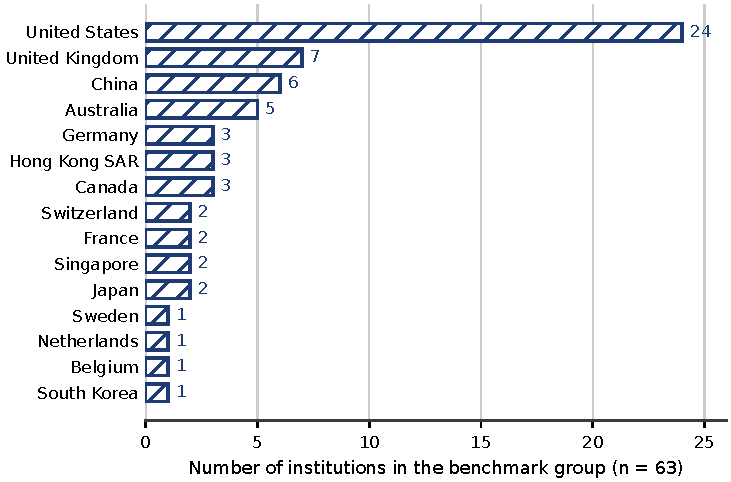
\includegraphics[width=\textwidth]{fig_countries.pdf}
	\caption{Composici\'on del grupo de referencia por pa\'is. El grupo es la cola superior extrema de tres clasificaciones internacionales y no es una muestra de las universidades del mundo; v\'ease la Secci\'on~\ref{sec:methods-design}.}\label{fig:paises}
\end{figure*}

\begin{figure*}[htbp]
	\centering
	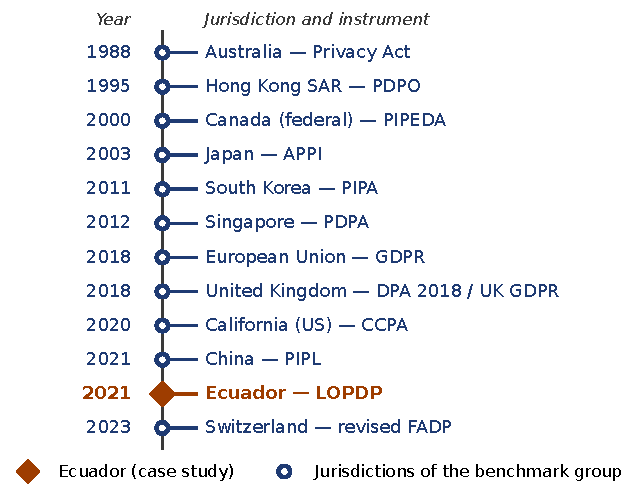
\includegraphics[width=\textwidth]{fig_timeline.pdf}
	\caption{A\~no en que entr\'o en vigor el r\'egimen general de protecci\'on de datos vigente en cada jurisdicci\'on del estudio. Para Estados Unidos, que carece de ley federal integral, se usa la CCPA de California. Ecuador pertenece a la oleada m\'as reciente, junto con China.}\label{fig:cronologia}
\end{figure*}

\end{appendices}

\bibliography{privacidad_mundo}

\end{document}
